\documentclass[14pt,a4paper]{extarticle}

% --- 1. Поддержка кириллицы, кодировок и шрифтов (СТП 01-2017) ---
\usepackage{cmap}
\usepackage[T2A]{fontenc}
\usepackage[utf8]{inputenc}
\usepackage[russian]{babel}
\usepackage{tempora} % Истинный Times New Roman для кириллицы и латиницы (с полной поддержкой Bold/Italic)

% --- 2. Геометрия страницы по СТП 01-2017 и образцу ОтчетRest.docx (Левое 30мм, Правое 15мм, Верхнее 20мм, Нижнее 20мм) ---
\usepackage[a4paper, left=30mm, right=15mm, top=20mm, bottom=20mm]{geometry}

% --- 3. Межстрочный интервал (полуторный) и абзацный отступ (1.25 см) ---
\usepackage{setspace}
\setstretch{1.25}
\usepackage{indentfirst}
\setlength{\parindent}{1.25cm}
\setlength{\parskip}{0pt}

% --- 4. Предотвращение выезда длинных слов и идентификаторов за границы листа ---
\sloppy
\emergencystretch=2.5em
\righthyphenmin=2
\lefthyphenmin=2

% --- 5. Математические пакеты и таблицы ---
\usepackage{amsmath,amssymb}
\usepackage{array}
\usepackage{tabularx}
\usepackage{booktabs}
\usepackage{graphicx}
\usepackage{float}
\usepackage{caption}

% --- 6. Оформление подписей к рисункам и таблицам по СТП 01-2017 (длинное тире) ---
\DeclareCaptionLabelSeparator{emdash}{~---~}
\captionsetup[figure]{name=Рисунок, labelsep=emdash, justification=centering, font=normalfont, size=normalsize}
\captionsetup[table]{name=Таблица, labelsep=emdash, justification=raggedright, singlelinecheck=false, font=normalfont, size=normalsize}

% --- 7. Оформление заголовков разделов и подразделов по СТП 01-2017 (14pt, абзацный отступ 1.25 см) ---
\usepackage{titlesec}
\titleformat{\section}[block]{\bfseries\normalsize\raggedright}{\thesection}{1em}{\MakeUppercase}
\titleformat{\subsection}[block]{\bfseries\normalsize\raggedright}{\thesubsection}{1em}{}
\titleformat{\subsubsection}[block]{\bfseries\normalsize\raggedright}{\thesubsubsection}{1em}{}

\titlespacing*{\section}{\parindent}{18pt}{18pt}
\titlespacing*{\subsection}{\parindent}{18pt}{18pt}
\titlespacing*{\subsubsection}{\parindent}{18pt}{18pt}

% --- 8. Листинги кода по СТП 01-2017 (без номеров строк слева, с рамкой и переносом) ---
\usepackage{fvextra}
\usepackage{fancyvrb}
\DefineVerbatimEnvironment{CodeListing}{Verbatim}{
    fontsize=\fontsize{9.5pt}{11.5pt}\selectfont,
    framesep=2.5mm,
    framerule=0.5pt,
    breaklines=true,
    breaksymbol={\tiny\ensuremath{\hookrightarrow}},
    xleftmargin=0pt,
    xrightmargin=0pt
}

% --- 9. Списки: отступы и стиль маркированных списков (маркер-дефис -) ---
\usepackage{enumitem}
\setlist{nosep, leftmargin=1.25cm}
\setlist[enumerate]{label=\arabic*., leftmargin=1.25cm}
\setlist[enumerate,1]{label=\arabic*., leftmargin=1.25cm}
\setlist[enumerate,2]{label=\arabic{enumi}.\arabic*., leftmargin=1.25cm}
\setlist[itemize]{label=-, leftmargin=1.25cm}
\renewcommand{\labelitemi}{-}
\renewcommand{\labelitemii}{-}

% --- 10. Нумерация страниц справа по СТП 01-2017 ---
\usepackage{fancyhdr}
\pagestyle{fancy}
\fancyhf{}
\fancyfoot[R]{\thepage}
\renewcommand{\headrulewidth}{0pt}
\renewcommand{\footrulewidth}{0pt}

\fancypagestyle{plain}{
    \fancyhf{}
    \fancyfoot[R]{\thepage}
    \renewcommand{\headrulewidth}{0pt}
    \renewcommand{\footrulewidth}{0pt}
}

\begin{document}

% ==============================================================================
% ТИТУЛЬНЫЙ ЛИСТ (образцу СТП 01-2017 и ЛР1, без слова вариант)
% ==============================================================================
\begin{titlepage}
    \begin{center}
        Министерство образования Республики Беларусь\\[0.15cm]
        Учреждение образования\\[0.15cm]
        «БЕЛОРУССКИЙ ГОСУДАРСТВЕННЫЙ УНИВЕРСИТЕТ\\
        ИНФОРМАТИКИ И РАДИОЭЛЕКТРОНИКИ»
    \end{center}
    
    \vspace{0.4cm}
    
    \begin{flushleft}
        Факультет компьютерных систем и сетей\\[0.1cm]
        Кафедра программного обеспечения информационных технологий\\[0.1cm]
        Дисциплина: Методы машинного обучения (ММО)
    \end{flushleft}
    
    \vspace{2.2cm}
    
    \begin{center}
        \large\textbf{ОТЧЕТ}\\[0.2cm]
        \normalsize
        {по лабораторной работе № 2}\\[0.3cm]
        Тема работы: Разведочный и предиктивный анализ данных
    \end{center}
    
    \vspace{2.5cm}
    
    \noindent
    \begin{tabular}{@{}p{0.62\textwidth}@{}p{0.38\textwidth}@{}}
        Выполнила: & \\
        студентка гр. 351002 & Алексейчик Я.\,Н. \\[0.5cm]
        Проверил: & Лебедевич А.\,В.
    \end{tabular}
    
    \vfill
    
    \begin{center}
        Минск 2026
    \end{center}
\end{titlepage}

\setcounter{page}{2}

% ==============================================================================
% 1 ЦЕЛЬ ВЫПОЛНЕНИЯ РАБОТЫ
% ==============================================================================
\section{Цель выполнения лабораторной работы}

Целью выполнения лабораторной работы является практическое освоение современных методов сбора, первичного разведочного анализа (Exploratory Data Analysis, EDA) и комплексной предобработки структурированных табличных данных для задач машинного обучения с использованием экосистемы Python (\texttt{pandas}, \texttt{numpy}, \texttt{scikit-learn}, \texttt{matplotlib}, \texttt{seaborn}):

\begin{enumerate}
    \item \textbf{Импорт и первичный структурный анализ выборки:} исследование схемы данных, определение размерности, разделение типов признаков на числовые и категориальные, вычисление фундаментальных параметров описательной статистики (математическое ожидание, дисперсия, квартили, размах).
    \item \textbf{Анализ и обработка пропущенных значений:} статистическая детекция скрытых пропусков (\texttt{NaN}), их визуализация тепловыми картами и столбчатыми диаграммами, обоснование и реализация математически корректной стратегии импутации модой для категориальных шкал с целью сохранения 100\% объема наблюдений; контрольная графическая верификация чистоты данных.
    \item \textbf{Обнаружение и устранение аномальных значений (выбросов):} расчет границ допустимого диапазона по правилу межквартильного размаха Дж. Тьюки ($1.5 \times IQR$), выявление логических противоречий в данных, визуализация аномалий на гистограммах и диаграммах размаха BoxPlot; устранение выбросов методом винсоризации (\textit{clipping}) без удаления строк; графическое подтверждение отсутствия выбросов.
    \item \textbf{Генерация новых признаков (Feature Engineering):} математический синтез 5 предметно-обоснованных характеристик (отношений, линейных взвешенных сверток, разностей прогресса и бинарных пороговых индикаторов) для обогащения признакового пространства и раскрытия нелинейных взаимосвязей.
    \item \textbf{Кодирование категориальных признаков:} приведение строковых данных к числовому матричному виду посредством трех методов: бинаризации дихотомических признаков (0 / 1), порядкового кодирования (Ordinal Encoding) для ранговых шкал (0, 1, 2) и прямого кодирования (One-Hot Encoding, OHE) для номинальных переменных с целью исключения фиктивного метрического порядка.
    \item \textbf{Масштабирование числовых признаков:} программная реализация нормализации (\texttt{MinMaxScaler}) в единичный диапазон $[0, 1]$ и стандартизации (\texttt{StandardScaler}) к нулевому среднему и единичной дисперсии; аналитическое и графическое сопоставление плотностей распределения (KDE), доказательство инвариантности топологии распределений при линейных трансформациях.
\end{enumerate}

% ==============================================================================
% 2 КРАТКИЕ ТЕОРЕТИЧЕСКИЕ СВЕДЕНИЯ
% ==============================================================================
\clearpage
\section{Краткие теоретические сведения}

\subsection{Концепция Exploratory Data Analysis (EDA) и предобработки данных}

В прикладном машинном обучении качество и надежность прогнозных моделей напрямую определяются качеством входных обучающих выборок. Принцип \textbf{«Garbage In --- Garbage Out»} (GIGO) констатирует, что даже архитектурно совершенный классификатор или регрессор при обучении на зашумленных данных с пропусками, несогласованными масштабами и выбросами выявит ложные корреляции и продемонстрирует низкую обобщающую способность.

Разведочный анализ данных (Exploratory Data Analysis, EDA) представляет собой формализованную методологию критического анализа выборок до построения предиктивных алгоритмов. EDA решает следующие ключевые задачи:
\begin{itemize}
    \item выявление внутренней геометрической структуры признакового пространства;
    \item локализация пропущенных значений и скрытых искажений;
    \item обнаружение экстремальных аномалий, деформирующих оптимизационный ландшафт функций потерь;
    \item преобразование качественных шкал в согласованные числовые тензоры;
    \item выравнивание масштабных коэффициентов признаков для обеспечения численной стабильности градиентных методов.
\end{itemize}

\subsection{Анализ и методы импутации пропущенных значений}

Пропуски в данных (\textit{Missing Values}) возникают вследствие сбоев опрашивающих систем, ошибок операторов, нежелания респондентов указывать конфиденциальные данные или потери сетевых пакетов. В математической статистике выделяют три фундаментальных механизма возникновения пропусков:
\begin{enumerate}
    \item \textbf{MCAR (Missing Completely at Random):} вероятность пропуска значения не зависит ни от наблюдаемых, ни от ненаблюдаемых признаков.
    \item \textbf{MAR (Missing at Random):} вероятность отсутствия значения признака $X$ систематически связана с другими известными признаками $Y$, но не с истинной величиной самого $X$.
    \item \textbf{MNAR (Missing Not at Random):} вероятность пропуска непосредственно детерминирована ненаблюдаемой величиной самого признака.
\end{enumerate}

\subsubsection{Стратегии обработки пропусков:}
\begin{itemize}
    \item \textbf{Полное удаление наблюдений (Listwise Deletion):} удаление любой строки, содержащей хотя бы один пропуск. Метод допустим только при доле поврежденных записей $<1\%$ и механизме MCAR. В противном случае происходит катастрофическая деградация статистической мощности выборки и смещение оценок.
    \item \textbf{Импутация средним или медианой:} эффективна для непрерывных числовых величин с нормальным или скошенным распределением соответственно.
    \item \textbf{Импутация модой (Mode Imputation):} замещение пропущенных значений наиболее частой категорией выборки. Для категориальной случайной величины $X$, принимающей значения из дискретного множества $C = \{c_1, \dots, c_k\}$, мода определяется как аргумент максимума эмпирической частоты:
    \begin{equation}
        M_0 = \arg\max_{c \in C} \sum_{i=1}^N \mathbb{I}(x_i = c),
    \end{equation}
    где $\mathbb{I}(\cdot)$ --- индикаторная функция. При работе с категориальными шкалами мода является единственной математически корректной мерой центральной тенденции, поскольку операции суммирования и деления для качественных меток не определены.
\end{itemize}

\subsection{Математический аппарат обнаружения выбросов по методу IQR}

\textbf{Выброс (Outlier)} --- это наблюдение, находящееся на аномально большом удалении от математического ожидания основной генеральной совокупности. Выбросы искажают оценки выборочной дисперсии, смещают разделяющие гиперплоскости линейных моделей и вызывают расходимость градиентного спуска.

Для устойчивого (\textit{robust}) поиска аномалий в распределениях применяется критерий Джона Тьюки, основанный на квантилях и \textbf{межквартильном размахе (Interquartile Range, IQR)}:
\begin{enumerate}
    \item Наблюдения упорядочиваются по возрастанию.
    \item Вычисляются первый квартиль $Q_1$ (25-й перцентиль) и третий квартиль $Q_3$ (75-й перцентиль):
    \begin{equation}
        P(X \le Q_1) = 0.25, \quad P(X \le Q_3) = 0.75.
    \end{equation}
    \item Межквартильный размах задает ширину диапазона, охватывающего 50\% центральной массы выборки:
    \begin{equation}
        IQR = Q_3 - Q_1.
    \end{equation}
    \item Границы статистически допустимых значений («усы» диаграммы размаха BoxPlot) определяются как:
    \begin{equation}
        X_{\text{нижн}} = Q_1 - 1.5 \times IQR, \quad X_{\text{верх}} = Q_3 + 1.5 \times IQR.
    \end{equation}
\end{enumerate}

Коэффициент 1.5 выбран исходя из свойств стандартного нормального распределения $\mathcal{N}(0, \sigma^2)$, где интервал $[Q_1 - 1.5 \times IQR, \; Q_3 + 1.5 \times IQR]$ соответствует диапазону $[\mu - 2.698\sigma, \; \mu + 2.698\sigma]$ и охватывает 99.3\% выборки, отсекая лишь крайние 0.7\% истинных хвостов.

\subsection{Методология устранения выбросов: винсоризация против удаления}

Выделяют два фундаментальных класса аномалий:
\begin{enumerate}
    \item \textbf{Логические ошибки ввода:} значения, нарушающие аксиоматику предметной области (например, балл за экзамен $101$ при допустимой шкале $[0, 100]$). Подлежат жесткой коррекции к предельно допустимому значению шкалы.
    \item \textbf{Экстремальные статистические выбросы:} реальные, но редкие наблюдения (например, 44 часа самостоятельной учебы в неделю при норме 20).
\end{enumerate}

Физическое удаление строк с выбросами (\textit{Trimming}) уменьшает размер выборки и удаляет ценную информацию по другим признакам данных студентов. В качестве математически обоснованной альтернативы применяется \textbf{винсоризация (Winsorization / Clipping)}: экстремальные значения за пределами интервала $[X_{\text{нижн}}, X_{\text{верх}}]$ принудительно ограничиваются граничными порогами:
\begin{equation}
    x_{\text{new}} = 
    \begin{cases}
        X_{\text{нижн}}, & \text{если } x < X_{\text{нижн}}, \\
        X_{\text{верх}}, & \text{если } x > X_{\text{верх}}, \\
        x, & \text{если } X_{\text{нижн}} \le x \le X_{\text{верх}}.
    \end{cases}
\end{equation}
Винсоризация гарантирует 100\% сохранность объема обучающей выборки, ликвидирует длинные тяжелые хвосты и предотвращает взрыв градиентов при обучении моделей.

\subsection{Инженерия признаков (Feature Engineering)}

\textbf{Feature Engineering} --- это целенаправленное конструирование новых математических атрибутов на основе исходных переменных выборки с использованием предметных закономерностей. Введение явных функциональных преобразований позволяет:
\begin{itemize}
    \item выразить относительные пропорции и баланс распределения ресурсов (отношение учебы ко сну);
    \item объединить гетерогенные характеристики в единый комплексный взвешенный индекс усилий;
    \item зафиксировать динамику изменения процесса (прирост экзаменационного балла относительно прошлых тестов);
    \item дискретизировать ключевые пороговые эффекты (индикатор высокой посещаемости).
\end{itemize}

\subsection{Математические методы кодирования категориальных данных}

Компьютерные алгоритмы машинного обучения оперируют матрицами вещественных чисел. Преобразование текстовых категорий требует строгого учета характера статистической шкалы:

\begin{enumerate}
    \item \textbf{Бинаризация (Binary Encoding):} применяется для дихотомических признаков, принимающих ровно два взаимоисключающих значения ($C = \{c_0, c_1\}$):
    \begin{equation}
        f(x) = \begin{cases} 0, & \text{если } x = c_0, \\ 1, & \text{если } x = c_1. \end{cases}
    \end{equation}
    \item \textbf{Порядковое кодирование (Ordinal Encoding):} применяется для ранговых шкал, обладающих естественным монотонным отношением порядка ($c_0 < c_1 < \dots < c_{k-1}$):
    \begin{equation}
        f(c_j) = j, \quad j \in \{0, 1, \dots, k-1\}.
    \end{equation}
    Метод сохраняет транзитивность отношений и порядок интенсивности признака.
    \item \textbf{Прямое унитарное кодирование (One-Hot Encoding, OHE):} применяется для номинальных признаков, категории которых равноправны и не имеют физического порядка (например, тип влияния сверстников). Номинальный признак с $k$ уникальными градациями раскладывается на $k$ бинарных векторных индикаторов:
    \begin{equation}
        \mathbf{e}_j = (0, \dots, 0, \underbrace{1}_{j\text{-я позиция}}, 0, \dots, 0)^T.
    \end{equation}
    OHE исключает ложное предположение линейных моделей о том, что категория с кодом 2 «больше» категории с кодом 1.
\end{enumerate}

\subsection{Масштабирование числовых признаков: нормализация и стандартизация}

В работе исследованы и применены два метода масштабирования:
\begin{enumerate}
    \item \textbf{Нормализация (Min-Max Scaling):} линейное сжатие непрерывной шкалы строго в отрезок $[0, 1]$:
    \begin{equation}
        X_{\text{norm}} = \frac{X - X_{\min}}{X_{\max} - X_{\min}}.
    \end{equation}
    \item \textbf{Стандартизация (Z-Score Standardization):} аффинное центрирование признака к нулевому выборочному среднему ($\mu = 0$) и масштабирование к единичному стандартному отклонению ($\sigma = 1$):
    \begin{equation}
        X_{\text{std}} = \frac{X - \mu}{\sigma}, \quad \mu = \frac{1}{N}\sum_{i=1}^N x_i, \quad \sigma = \sqrt{\frac{1}{N}\sum_{i=1}^N (x_i - \mu)^2}.
    \end{equation}
\end{enumerate}

\textbf{Теорема об инвариантности плотности распределения:} Пусть случайная величина $X$ имеет непрерывную функцию плотности вероятностей $p_X(x)$. Линейное преобразование $Y = aX + b$ (где $a > 0$) формирует новую случайную величину $Y$ с плотностью:
\begin{equation}
    p_Y(y) = \frac{1}{a} p_X\left(\frac{y - b}{a}\right).
\end{equation}
Поскольку формулы \texttt{MinMaxScaler} ($a = \frac{1}{X_{\max}-X_{\min}}$, $b = -\frac{X_{\min}}{X_{\max}-X_{\min}}$) и \texttt{StandardScaler} ($a = \frac{1}{\sigma}$, $b = -\frac{\mu}{\sigma}$) представляют собой строго линейные преобразования с положительным множителем $a > 0$, они выполняют лишь масштабное сжатие и параллельный перенос вдоль оси абсцисс. Коэффициент асимметрии (\textit{Skewness}), эксцесс (\textit{Kurtosis}) и геометрическая форма ядерной оценки плотности (KDE) остаются абсолютно инвариантными.

% ==============================================================================
% 3 ФОРМУЛИРОВКА ЗАДАНИЯ
% ==============================================================================
\clearpage
\section{Формулировка задания}

В соответствии с официальной рабочей программой дисциплины «Методы машинного обучения» кафедры ПОИТ сформулировано следующее комплексное задание на лабораторную работу:

\begin{enumerate}
    \item \textbf{Импортировать датасет.} Выбрать исходный структурированный массив данных (самостоятельно с портала \texttt{kaggle.com} либо из прикрепленных файлов учебно-методического комплекса).
    \item \textbf{Провести очистку и разведочный анализ:}
    \begin{enumerate}
        \item Проверить данные на пропуски и наличие аномальных значений с использованием статистических критериев и графических средств визуализации (графики распределений, столбчатые диаграммы, графики типа BoxPlot, тепловые карты).
        \item Заполнить пропуски научно обоснованными методами и устранить выявленные выбросы.
        \item Графически подтвердить полное отсутствие пропусков и аномальных значений после выполнения процедур очистки.
    \end{enumerate}
    \item \textbf{Инженерия признаков и кодирование:}
    \begin{enumerate}
        \item Сгенерировать новые признаки (не менее двух предметно-обоснованных переменных).
        \item Применить математически корректное кодирование качественных категориальных признаков (бинаризация дихотомических признаков, порядковое кодирование ранговых категорий, One-Hot кодирование номинальных факторов).
    \end{enumerate}
    \item \textbf{Масштабирование данных:} выполнить стандартизацию и/или нормализацию числовых признаков; провести сопоставительный анализ распределений до и после масштабирования.
\end{enumerate}

\subsection{Спецификация исследуемого датасета}

В качестве объекта исследования выбран массив данных \textbf{«Student Performance Factors»} (\texttt{StudentPerformanceFactors.csv}), содержащий комплексные академические, психологические, бытовые и социально-демографические параметры 6607 студентов, а также их итоговые результаты на экзамене (\texttt{Exam\_Score}). Исходная матрица данных имеет размерность: \textbf{6607 строк и 20 столбцов} (19 признаков-предикторов и 1 целевая переменная). Подробная спецификация признаков приведена в таблице~\ref{tab:features_spec}.

\begin{table}[H]
    \centering
    \caption{Спецификация признаков датасета Student Performance Factors}
    \label{tab:features_spec}
    \fontsize{8.5pt}{10.5pt}\selectfont
    \begin{tabularx}{\textwidth}{|c|>{\raggedright\arraybackslash}p{3.8cm}|c|c|>{\raggedright\arraybackslash}X|}
        \hline
        \textbf{№} & \textbf{Идентификатор} & \textbf{Тип данных} & \textbf{Роль} & \textbf{Предметно-содержательное описание} \\
        \hline
        1 & \texttt{Hours\_Studied} & \texttt{int64} & Фактор & Часов самостоятельной учебы в неделю \\
        \hline
        2 & \texttt{Attendance} & \texttt{int64} & Фактор & Процент посещаемости учебных занятий (0--100\%) \\
        \hline
        3 & \texttt{Parental\_Involvement} & \texttt{object} (str) & Фактор & Вовлеченность родителей ('Low', 'Medium', 'High') \\
        \hline
        4 & \texttt{Access\_to\_Resources} & \texttt{object} (str) & Фактор & Доступность ресурсов ('Low', 'Medium', 'High') \\
        \hline
        5 & \texttt{Extracurricular\_Activities} & \texttt{object} (str) & Фактор & Внеучебная активность ('No', 'Yes') \\
        \hline
        6 & \texttt{Sleep\_Hours} & \texttt{int64} & Фактор & Среднее количество часов сна в сутки (4--10) \\
        \hline
        7 & \texttt{Previous\_Scores} & \texttt{int64} & Фактор & Результаты прошлых тестирований (50--100) \\
        \hline
        8 & \texttt{Motivation\_Level} & \texttt{object} (str) & Фактор & Уровень мотивации ('Low', 'Medium', 'High') \\
        \hline
        9 & \texttt{Internet\_Access} & \texttt{object} (str) & Фактор & Наличие интернета дома ('No', 'Yes') \\
        \hline
        10 & \texttt{Tutoring\_Sessions} & \texttt{int64} & Фактор & Число занятий с репетитором в месяц (0--8) \\
        \hline
        11 & \texttt{Family\_Income} & \texttt{object} (str) & Фактор & Доход семьи ('Low', 'Medium', 'High') \\
        \hline
        12 & \texttt{Teacher\_Quality} & \texttt{object} (str) & Фактор & Оценка квалификации учителей ('Low', 'Med', 'High') \\
        \hline
        13 & \texttt{School\_Type} & \texttt{object} (str) & Фактор & Тип учебного заведения ('Public', 'Private') \\
        \hline
        14 & \texttt{Peer\_Influence} & \texttt{object} (str) & Фактор & Влияние окружения ('Positive', 'Neutral', 'Negative') \\
        \hline
        15 & \texttt{Physical\_Activity} & \texttt{int64} & Фактор & Часов спорта в неделю (0--6) \\
        \hline
        16 & \texttt{Learning\_Disabilities} & \texttt{object} (str) & Фактор & Трудности в обучении ('No', 'Yes') \\
        \hline
        17 & \texttt{Parental\_Education\_Level} & \texttt{object} (str) & Фактор & Образование родителей ('High School', 'College', ...) \\
        \hline
        18 & \texttt{Distance\_from\_Home} & \texttt{object} (str) & Фактор & Удаленность от школы ('Near', 'Moderate', 'Far') \\
        \hline
        19 & \texttt{Gender} & \texttt{object} (str) & Фактор & Пол обучающегося ('Male', 'Female') \\
        \hline
        20 & \texttt{Exam\_Score} & \texttt{int64} & \textbf{Целевой} & Итоговый балл студента на экзамене (0--100) \\
        \hline
    \end{tabularx}
\end{table}

\subsection{Матрица верификации выполнения требований задания}

В таблице~\ref{tab:compliance_matrix} представлено прямое сопоставление нормативных пунктов задания кафедры с фактически реализованными модулями программного комплекса.

\begin{table}[H]
    \centering
    \caption{Матрица верификации соответствия работы официальному заданию}
    \label{tab:compliance_matrix}
    \fontsize{8.5pt}{10.5pt}\selectfont
    \begin{tabularx}{\textwidth}{|>{\raggedright\arraybackslash}p{2.8cm}|>{\raggedright\arraybackslash}p{4.2cm}|>{\raggedright\arraybackslash}X|>{\centering\arraybackslash}p{2.0cm}|}
        \hline
        \textbf{Пункт задания} & \textbf{Нормативное требование} & \textbf{Фактическая реализация в проекте} & \textbf{Статус} \\
        \hline
        1. Импорт данных & Загрузка табличного массива & Модуль \texttt{data\_loader.py}, функция \texttt{load\_dataset()}, 6607 строк, 20 столбцов & Выполнено \\
        \hline
        2. Анализ пропусков & Статистический и визуальный поиск \texttt{NaN} & \texttt{get\_missing\_summary()}, Рис.~\ref{fig:miss_before} (Heatmap) и Рис.~\ref{fig:miss_bar} (Bar chart) & Выполнено \\
        \hline
        2. Заполнение пропусков & Устранение выявленных пропусков & \texttt{impute\_missing\_with\_mode()}: категориальные признаки заполнены модой & Выполнено \\
        \hline
        2. Контроль пропусков & Графическая верификация чистоты данных & Повторный Heatmap (Рис.~\ref{fig:miss_after}) с бейджем «100\% заполненность» (0 пропусков) & Выполнено \\
        \hline
        2. Анализ выбросов & Расчет статистик и графики распределений & Расчет границ $1.5 \times IQR$, Рис.~\ref{fig:dist_before} (Hist+KDE), Рис.~\ref{fig:box_before} (BoxPlot) & Выполнено \\
        \hline
        2. Устранение выбросов & Ликвидация аномалий и артефактов & Коррекция ошибки 101 балл, винсоризация (\texttt{clip}) по границам $IQR$ & Выполнено \\
        \hline
        2. Контроль выбросов & Графическая проверка отсутствия аномалий & Контрольные BoxPlot (Рис.~\ref{fig:box_after}), гистограммы (Рис.~\ref{fig:dist_after}), матрица корреляций (Рис.~\ref{fig:corr}) & Выполнено \\
        \hline
        3. Feature Engineering & Генерация $\ge 2$ новых признаков & Синтезировано \textbf{5 предметных признаков} в \texttt{feature\_engineering.py}, Рис.~\ref{fig:fe} & Выполнено \\
        \hline
        3. Кодирование категорий & OHE, бинаризация и другие методы & Бинаризация 5 колонок, Ordinal 7 колонок, One-Hot 1 колонки (итого 27 признаков) & Выполнено \\
        \hline
        4. Масштабирование данных & Стандартизация и/или нормализация & Реализованы \texttt{MinMaxScaler} и \texttt{StandardScaler}, Рис.~\ref{fig:scaling} (сравнение KDE) & Выполнено \\
        \hline
    \end{tabularx}
\end{table}

% ==============================================================================
% 4 ВЕСЬ КОД РЕШЕНИЯ ЛАБОРАТОРНОЙ РАБОТЫ
% ==============================================================================
\clearpage
\section{Весь код решения лабораторной работы}

\subsection{Исходный код модуля конфигурации (файл config.py)}
\begin{CodeListing}
# -*- coding: utf-8 -*-
"""
Модуль конфигурации лабораторной работы No.  2.
Определяет файловые пути, глобальные константы и словари кодирования категорий.
"""

import os
from typing import Dict

# Базовые пути проекта
BASE_DIR: str = os.path.dirname(os.path.abspath(__file__))
DATASET_PATH: str = os.path.abspath(
    os.path.join(
        BASE_DIR, '..', 'Задание', 'StudentPerformanceFactors',
        'StudentPerformanceFactors.csv'
    )
)
IMAGES_DIR: str = os.path.join(BASE_DIR, 'images')
PROCESSED_DATA_DIR: str = os.path.join(BASE_DIR, 'processed_data')

REPORT_DIR: str = os.path.abspath(os.path.join(BASE_DIR, '..', 'Отчет'))
REPORT_IMAGES_DIR: str = os.path.join(REPORT_DIR, 'images')
REPORT_OVERLEAF_IMAGES_DIR: str = os.path.join(
    REPORT_DIR, 'Отчет_Overleaf', 'images'
)

# Словари для бинаризации категориальных признаков (0 / 1)
BINARY_MAPPINGS: Dict[str, Dict[str, int]] = {
    'Extracurricular_Activities': {'No': 0, 'Yes': 1},
    'Internet_Access': {'No': 0, 'Yes': 1},
    'Learning_Disabilities': {'No': 0, 'Yes': 1},
    'School_Type': {'Public': 0, 'Private': 1},
    'Gender': {'Male': 0, 'Female': 1}
}

# Словари для порядкового кодирования (Ordinal Encoding)
ORDINAL_MAPPINGS: Dict[str, Dict[str, int]] = {
    'Parental_Involvement': {'Low': 0, 'Medium': 1, 'High': 2},
    'Access_to_Resources': {'Low': 0, 'Medium': 1, 'High': 2},
    'Motivation_Level': {'Low': 0, 'Medium': 1, 'High': 2},
    'Family_Income': {'Low': 0, 'Medium': 1, 'High': 2},
    'Teacher_Quality': {'Low': 0, 'Medium': 1, 'High': 2},
    'Distance_from_Home': {'Near': 0, 'Moderate': 1, 'Far': 2},
    'Parental_Education_Level': {
        'High School': 0,
        'College': 1,
        'Postgraduate': 2
    }
}

# Признаки для One-Hot кодирования
OHE_COLUMNS: list[str] = ['Peer_Influence']

# Непрерывные числовые признаки для стандартизации и нормализации
CONTINUOUS_COLUMNS_TO_SCALE: list[str] = [
    'Hours_Studied', 'Attendance', 'Sleep_Hours', 'Previous_Scores',
    'Tutoring_Sessions', 'Physical_Activity', 'Exam_Score',
    'Study_Sleep_Ratio', 'Total_Study_Effort', 'Score_Improvement',
    'Physical_Study_Balance'
]

# Ключевые демонстрационные признаки для детального анализа распределений

DEMO_COLUMNS: list[str] = [
    'Hours_Studied', 'Attendance', 'Exam_Score', 'Total_Study_Effort'
]\end{CodeListing}

\clearpage
\subsection{Исходный код модуля загрузки данных (файл data\_loader.py)}
\begin{CodeListing}
# -*- coding: utf-8 -*-
"""
Модуль загрузки и первичного осмотра данных.
"""

from typing import List, Tuple
import numpy as np
import pandas as pd


def load_dataset(filepath: str) -> pd.DataFrame:
    """
    Загружает CSV датасет в pandas DataFrame.

    :param filepath: Абсолютный или относительный путь к CSV-файлу.
    :return: DataFrame с загруженными данными.
    :raises FileNotFoundError: Если файл не найден.
    """
    return pd.read_csv(filepath)


def get_column_types(df: pd.DataFrame) -> Tuple[List[str], List[str]]:
    """
    Разделяет признаки датасета на числовые и категориальные.

    :param df: Исходный датасет.
    :return: Кортеж (числовые_колонки, категориальные_колонки).
    """
    numeric_cols = df.select_dtypes(include=[np.number]).columns.tolist()
    categorical_cols = df.select_dtypes(exclude=[np.number]).columns.tolist()
    return numeric_cols, categorical_cols


def get_numeric_summary(
    df: pd.DataFrame, numeric_cols: List[str]
) -> pd.DataFrame:
    """
    Формирует таблицу описательных статистик для числовых колонок.

    :param df: Исходный датасет.
    :param numeric_cols: Список числовых признаков.
    :return: Транспонированный DataFrame со статистиками.
    """
    cols_to_show = [
        'count', 'mean', 'std', 'min', '25%', '50%', '75%', 'max'
    ]
    return df[numeric_cols].describe().round(2).T[cols_to_show]\end{CodeListing}

\clearpage
\subsection{Исходный код модуля очистки данных и обработки выбросов (файл preprocessor.py)}
\begin{CodeListing}
# -*- coding: utf-8 -*-
"""
Модуль предварительной очистки данных:
- Обнаружение и импутация пропущенных значений модой
- Расчет статистических границ по формуле межквартильного размаха (IQR)
- Устранение логических аномалий и винсоризация (clipping) выбросов
"""

from typing import Dict, List, Tuple
import pandas as pd


def get_missing_summary(df: pd.DataFrame) -> pd.DataFrame:
    """
    Вычисляет количество и процентное соотношение пропусков в столбцах.

    :param df: Анализируемый DataFrame.
    :return: DataFrame с колонками 'Пропусков (шт.)' и 'Процент (%)'.
    """
    missing_counts = df.isnull().sum()
    missing_pct = (missing_counts / len(df) * 100).round(2)
    summary = pd.DataFrame({
        'Пропусков (шт.)': missing_counts,
        'Процент (%)': missing_pct
    })
    return summary[summary['Пропусков (шт.)'] > 0].sort_values(
        by='Пропусков (шт.)', ascending=False
    )


def impute_missing_with_mode(
    df: pd.DataFrame, columns: List[str]
) -> Tuple[pd.DataFrame, Dict[str, str]]:
    """
    Заполняет пропущенные значения категориальных признаков их модой.

    :param df: Исходный датасет.
    :param columns: Список колонок для заполнения.
    :return: Кортеж (очищенный DataFrame, словарь подставленных мод).
    """
    df_clean = df.copy()
    imputed_modes: Dict[str, str] = {}
    for col in columns:
        if df_clean[col].isnull().any():
            mode_val = str(df_clean[col].mode()[0])
            imputed_modes[col] = mode_val
            df_clean[col] = df_clean[col].fillna(mode_val)
    return df_clean, imputed_modes


def calculate_iqr_bounds(
    df: pd.DataFrame, numeric_cols: List[str]
) -> Tuple[pd.DataFrame, Dict[str, Tuple[float, float]]]:
    """
    Рассчитывает статистические границы выбросов по правилу 1.5 * IQR.

    :param df: Анализируемый DataFrame.
    :param numeric_cols: Список числовых признаков.
    :return: Таблица статистик выбросов и словарь {признак: (нижняя, верхняя)}.
    """
    outlier_stats = []
    bounds_dict: Dict[str, Tuple[float, float]] = {}

    for col in numeric_cols:
        q1 = float(df[col].quantile(0.25))
        q3 = float(df[col].quantile(0.75))
        iqr = q3 - q1
        lower = q1 - 1.5 * iqr
        upper = q3 + 1.5 * iqr
        bounds_dict[col] = (lower, upper)

        outliers_count = int(
            ((df[col] < lower) | (df[col] > upper)).sum()
        )
        pct = (outliers_count / len(df) * 100)

        outlier_stats.append({
            'Признак': col,
            'Q1': q1,
            'Q3': q3,
            'IQR': iqr,
            'Нижняя граница': lower,
            'Верхняя граница': upper,
            'Мин. значение': float(df[col].min()),
            'Макс. значение': float(df[col].max()),
            'Кол-во выбросов': outliers_count,
            'Процент (%)': round(pct, 2)
        })

    summary_df = pd.DataFrame(outlier_stats).set_index('Признак')
    return summary_df, bounds_dict


def handle_outliers(
    df: pd.DataFrame,
    bounds_dict: Dict[str, Tuple[float, float]],
    target_cols: List[str]
) -> pd.DataFrame:
    """
    Устраняет логические аномалии и применяет винсоризацию (clipping)
    к числовым признакам с выбросами.

    :param df: Исходный датасет.
    :param bounds_dict: Словарь с границами IQR.
    :param target_cols: Признаки, подлежащие винсоризации.
    :return: DataFrame с устраненными выбросами.
    """
    df_clean = df.copy()

    # 1. Корректировка логической аномалии: Exam_Score > 100
    if 'Exam_Score' in df_clean.columns:
        df_clean.loc[df_clean['Exam_Score'] > 100, 'Exam_Score'] = 100

    # 2. Винсоризация (clipping)
    for col in target_cols:
        low, high = bounds_dict[col]
        # Нижняя граница не может быть отрицательной для счетчиков занятий
        low = max(low, 0.0)
        # Верхняя граница экзамена не выше 100
        if col == 'Exam_Score':
            high = min(high, 100.0)

        df_clean[col] = df_clean[col].clip(lower=low, upper=high)

    return df_clean\end{CodeListing}

\clearpage
\subsection{Исходный код модуля генерации признаков и кодирования (файл feature\_engineering.py)}
\begin{CodeListing}
# -*- coding: utf-8 -*-
"""
Модуль генерации новых признаков (Feature Engineering)
и кодирования категориальных переменных.
"""

from typing import Dict, List, Tuple
import pandas as pd


def generate_new_features(
    df: pd.DataFrame
) -> Tuple[pd.DataFrame, List[str]]:
    """
    Генерирует 5 новых предметных признаков для повышения
    предсказательной способности моделей.

    :param df: Очищенный DataFrame.
    :return: Кортеж (DataFrame с новыми признаками, список имен признаков).
    """
    df_feat = df.copy()

    # 1. Study_Sleep_Ratio: баланс учебы и сна
    df_feat['Study_Sleep_Ratio'] = (
        df_feat['Hours_Studied'] / df_feat['Sleep_Hours']
    ).round(3)

    # 2. Total_Study_Effort: совокупные академические усилия
    df_feat['Total_Study_Effort'] = (
        df_feat['Hours_Studied']
        + 2.0 * df_feat['Tutoring_Sessions']
        + 0.1 * df_feat['Attendance']
    ).round(2)

    # 3. Score_Improvement: академический прогресс относительно прошлого уровня
    df_feat['Score_Improvement'] = (
        df_feat['Exam_Score'] - df_feat['Previous_Scores']
    ).round(2)

    # 4. Physical_Study_Balance: баланс спорта и учебной нагрузки
    df_feat['Physical_Study_Balance'] = (
        df_feat['Physical_Activity'] / (df_feat['Hours_Studied'] + 1)
    ).round(3)

    # 5. High_Attendance_Flag: бинарный флаг дисциплины (посещаемость >= 85%)
    df_feat['High_Attendance_Flag'] = (
        df_feat['Attendance'] >= 85
    ).astype(int)

    new_feature_names = [
        'Study_Sleep_Ratio',
        'Total_Study_Effort',
        'Score_Improvement',
        'Physical_Study_Balance',
        'High_Attendance_Flag'
    ]
    return df_feat, new_feature_names


def encode_binary_features(
    df: pd.DataFrame,
    mappings: Dict[str, Dict[str, int]]
) -> pd.DataFrame:
    """
    Выполняет бинаризацию дихотомических признаков (отображение в 0 и 1).

    :param df: DataFrame с категориальными признаками.
    :param mappings: Словарь {имя_колонки: {значение: 0_или_1}}.
    :return: Преобразованный DataFrame.
    """
    df_encoded = df.copy()
    for col, mapping in mappings.items():
        if col in df_encoded.columns:
            df_encoded[col] = df_encoded[col].map(mapping)
    return df_encoded


def encode_ordinal_features(
    df: pd.DataFrame,
    mappings: Dict[str, Dict[str, int]]
) -> pd.DataFrame:
    """
    Выполняет порядковое кодирование (Ordinal Encoding) ранговых категорий.

    :param df: DataFrame с категориальными признаками.
    :param mappings: Словарь {имя_колонки: {категория: ранг}}.
    :return: Преобразованный DataFrame.
    """
    df_encoded = df.copy()
    for col, mapping in mappings.items():
        if col in df_encoded.columns:
            df_encoded[col] = df_encoded[col].map(mapping)
    return df_encoded


def encode_nominal_features(
    df: pd.DataFrame,
    columns: List[str]
) -> Tuple[pd.DataFrame, List[str]]:
    """
    Выполняет One-Hot Encoding (OHE) для номинальных категориальных признаков.

    :param df: DataFrame.
    :param columns: Список номинальных признаков для прямого кодирования.
    :return: Кортеж (DataFrame с OHE-колонками, список добавленных имен).
    """
    df_encoded = pd.get_dummies(
        df, columns=columns, prefix=columns, dtype=int
    )
    new_ohe_cols = [
        c for c in df_encoded.columns
        if any(c.startswith(f"{orig}_") for orig in columns)
    ]
    return df_encoded, new_ohe_cols\end{CodeListing}

\clearpage
\subsection{Исходный код модуля масштабирования (файл scaler.py)}
\begin{CodeListing}
# -*- coding: utf-8 -*-
"""
Модуль стандартизации и нормализации данных.
Реализует алгоритмы MinMaxScaler и StandardScaler,
а также сравнительный статистический анализ.
"""

from typing import Dict, List
import pandas as pd
from sklearn.preprocessing import MinMaxScaler, StandardScaler


def apply_minmax_scaling(
    df: pd.DataFrame, columns: List[str]
) -> pd.DataFrame:
    """
    Выполняет нормализацию числовых признаков в диапазон [0, 1].

    :param df: Исходный DataFrame.
    :param columns: Список колонок для масштабирования.
    :return: DataFrame с нормализованными признаками.
    """
    df_scaled = df.copy()
    scaler = MinMaxScaler()
    df_scaled[columns] = scaler.fit_transform(df[columns])
    return df_scaled


def apply_standard_scaling(
    df: pd.DataFrame, columns: List[str]
) -> pd.DataFrame:
    """
    Выполняет стандартизацию признаков к mean=0 и std=1 (Z-score).

    :param df: Исходный DataFrame.
    :param columns: Список колонок для масштабирования.
    :return: DataFrame со стандартизированными признаками.
    """
    df_scaled = df.copy()
    scaler = StandardScaler()
    df_scaled[columns] = scaler.fit_transform(df[columns])
    return df_scaled


def compare_scaling_stats(
    df_orig: pd.DataFrame,
    df_minmax: pd.DataFrame,
    df_std: pd.DataFrame,
    columns: List[str]
) -> Dict[str, pd.DataFrame]:
    """
    Формирует сравнительные таблицы статистических параметров
    до и после различных методов масштабирования.

    :param df_orig: Исходный DataFrame.
    :param df_minmax: DataFrame после MinMaxScaler.
    :param df_std: DataFrame после StandardScaler.
    :param columns: Список анализируемых колонок.
    :return: Словарь {признак: сводная_таблица}.
    """
    results: Dict[str, pd.DataFrame] = {}
    metric_names = [
        'Среднее (Mean)', 'Станд. откл. (Std)',
        'Минимум (Min)', 'Максимум (Max)'
    ]

    for col in columns:
        col_comparison = pd.DataFrame({
            'Оригинал': [
                df_orig[col].mean(), df_orig[col].std(),
                df_orig[col].min(), df_orig[col].max()
            ],
            'MinMaxScaler': [
                df_minmax[col].mean(), df_minmax[col].std(),
                df_minmax[col].min(), df_minmax[col].max()
            ],
            'StandardScaler': [
                df_std[col].mean(), df_std[col].std(),
                df_std[col].min(), df_std[col].max()
            ]
        }, index=metric_names)
        results[col] = col_comparison.round(4)

    return results\end{CodeListing}

\clearpage
\subsection{Исходный код модуля расширенной визуализации (файл visualizer.py)}
\begin{CodeListing}
# -*- coding: utf-8 -*-
"""
Модуль расширенной графической визуализации данных.
Создает информативные, наглядные и эстетичные диаграммы с аннотациями,
статистическими сводками и поддержкой кириллицы.
"""

from typing import Dict, List, Optional, Tuple
import matplotlib
import matplotlib.pyplot as plt
import numpy as np
import pandas as pd
import seaborn as sns

matplotlib.use("Agg")

# Глобальная настройка типографики и стилей
plt.rcParams["font.sans-serif"] = ["DejaVu Sans", "Arial", "Liberation Sans"]
plt.rcParams["axes.unicode_minus"] = False
sns.set_theme(style="whitegrid", font="DejaVu Sans")


def plot_missing_heatmap(df: pd.DataFrame, title: str, save_path: str) -> None:
    """
    Строит наглядную тепловую карту пропущенных значений.
    """
    plt.figure(figsize=(14, 6))
    missing_sum = int(df.isnull().sum().sum())

    cmap = sns.color_palette(["#1f77b4", "#d62728"], as_cmap=True)
    ax = sns.heatmap(
        df.isnull(),
        cbar=True,
        yticklabels=False,
        cmap=cmap,
        vmin=0,
        vmax=1,
        cbar_kws={"label": "Наличие пропуска (0 - нет, 1 - да)", "ticks": [0, 1]},
    )

    # Настройка подписей шкалы (colorbar)
    cbar = ax.collections[0].colorbar
    if cbar:
        cbar.set_ticks([0, 1])
        cbar.set_ticklabels(["0 (Нет)", "1 (Пропуск)"])

    plt.title(
        f"{title}/n(Всего записей: {len(df):,}, суммарно пропусков: {missing_sum})",
        fontsize=14,
        fontweight="bold",
        pad=14,
    )
    plt.xlabel("Признаки датасета", fontsize=12, fontweight="bold", labelpad=10)
    plt.xticks(rotation=45, ha="right", fontsize=10)

    # Если пропусков 0, размещаем информационный бейдж по центру
    if missing_sum == 0:
        ax.text(
            0.5,
            0.5,
            "[OK] ПРОПУСКОВ НЕТ (100% заполненность выборки)",
            transform=ax.transAxes,
            fontsize=16,
            fontweight="bold",
            color="white",
            ha="center",
            va="center",
            bbox=dict(
                boxstyle="round,pad=0.8",
                facecolor="#2ca02c",
                edgecolor="none",
                alpha=0.9,
            ),
        )

    plt.tight_layout()
    plt.savefig(save_path, dpi=300)
    plt.close()


def plot_missing_bar(
    missing_table: pd.DataFrame,
    total_rows: int,
    save_path: str,
    imputed_modes: Optional[Dict[str, str]] = None,
) -> None:
    """
    Строит эстетичную горизонтальную диаграмму пропусков с точными числами,
    долями и планируемыми модальными значениями импутации.
    """
    fig, ax = plt.subplots(figsize=(10, 5))

    palette = sns.color_palette("rocket", n_colors=len(missing_table))
    y_pos = np.arange(len(missing_table))
    counts = missing_table["Пропусков (шт.)"].values

    bars = ax.barh(
        y_pos, counts, color=palette, height=0.55, edgecolor="black", linewidth=0.8
    )
    ax.set_yticks(y_pos)
    ax.set_yticklabels(missing_table.index, fontsize=11, fontweight="bold")
    ax.invert_yaxis()  # Самый частый пропуск вверху

    ax.set_xlabel("Количество пропущенных записей", fontsize=11, fontweight="bold")
    ax.set_title(
        "Количество и доля пропущенных значений по признакам/n"
        f"(Всего объектов выборки: {total_rows})",
        fontsize=13,
        fontweight="bold",
        pad=14,
    )

    # Добавляем текстовые аннотации к каждому столбцу
    for i, bar in enumerate(bars):
        w = bar.get_width()
        pct = (w / total_rows) * 100
        col_name = missing_table.index[i]
        mode_str = (
            f" | Мода: '{imputed_modes[col_name]}'"
            if (imputed_modes and col_name in imputed_modes)
            else ""
        )
        label_text = f" {int(w)} шт. ({pct:.2f}%){mode_str}"
        ax.text(
            w + 1.5,
            bar.get_y() + bar.get_height() / 2.0,
            label_text,
            va="center",
            ha="left",
            fontsize=10,
            fontweight="bold",
            color="#2c3e50",
        )

    ax.set_xlim(0, max(counts) * 1.35)
    plt.tight_layout()
    plt.savefig(save_path, dpi=300)
    plt.close()


def plot_distributions(
    df: pd.DataFrame,
    columns: List[str],
    title: str,
    save_path: str,
    color: str = "royalblue",
) -> None:
    """
    Строит сетку гистограмм с KDE, линиями среднего и медианы,
    а также карточками ключевых статистик для каждого признака.
    """
    fig, axes = plt.subplots(nrows=3, ncols=3, figsize=(16, 12))
    axes_flat = axes.flatten()

    for i, col in enumerate(columns):
        ax = axes_flat[i]
        data = df[col]
        mean_val = float(data.mean())
        median_val = float(data.median())
        std_val = float(data.std())
        skew_val = float(data.skew())

        # Гистограмма с KDE
        sns.histplot(
            data, kde=True, ax=ax, color=color, bins=20, edgecolor="white", alpha=0.65
        )

        # Вертикальные линии для Mean и Median
        ax.axvline(
            mean_val, color="#d62728", linestyle="--", linewidth=1.8, label=f"Mean: {
                mean_val:.1f}"
        )
        ax.axvline(
            median_val, color="#2ca02c", linestyle=":", linewidth=2.0, label=f"Median: {
                median_val:.1f}"
        )

        ax.set_title(f"Признак: {col}", fontsize=12, fontweight="bold", pad=8)
        ax.set_xlabel(col, fontsize=10)
        ax.set_ylabel("Частота", fontsize=10)
        ax.legend(loc="upper right", fontsize=8.5, framealpha=0.9)

        # Плашка со статистиками
        stats_text = f"Std: {std_val:.2f}/nSkew: {skew_val:+.2f}"
        ax.text(
            0.04,
            0.93,
            stats_text,
            transform=ax.transAxes,
            fontsize=8.5,
            verticalalignment="top",
            bbox=dict(
                boxstyle="round,pad=0.4",
                facecolor="white",
                edgecolor="gray",
                alpha=0.85,
            ),
        )

    # Удаление неиспользуемых осей
    for j in range(len(columns), len(axes_flat)):
        fig.delaxes(axes_flat[j])

    plt.suptitle(title, fontsize=15, fontweight="bold", y=0.99)
    plt.tight_layout()
    plt.savefig(save_path, dpi=300)
    plt.close()


def plot_boxplots(
    df: pd.DataFrame,
    columns: List[str],
    title: str,
    save_path: str,
    color: str = "salmon",
    bounds_dict: Optional[Dict[str, Tuple[float, float]]] = None,
) -> None:
    """
    Строит сетку BoxPlot с нанесением теоретических границ 1.5*IQR,
    маркерами среднего значения и подсчетом количества выбросов.
    """
    fig, axes = plt.subplots(nrows=2, ncols=4, figsize=(18, 9))
    axes_flat = axes.flatten()

    for i, col in enumerate(columns):
        ax = axes_flat[i]
        data = df[col]

        sns.boxplot(
            y=data,
            ax=ax,
            color=color,
            showmeans=True,
            meanprops=dict(
                marker="D",
                markeredgecolor="black",
                markerfacecolor="yellow",
                markersize=6,
            ),
            flierprops=dict(
                marker="o",
                markerfacecolor="#e74c3c",
                markeredgecolor="none",
                markersize=5,
                alpha=0.8,
            ),
        )

        ax.set_title(f"BoxPlot: {col}", fontsize=12, fontweight="bold", pad=8)
        ax.set_ylabel("Значение", fontsize=10)

        # Если переданы границы выбросов, наносим их пунктиром
        if bounds_dict and col in bounds_dict:
            low, high = bounds_dict[col]
            outliers_cnt = int(((data < low) | (data > high)).sum())

            # Линии границ
            ax.axhline(low, color="#c0392b", linestyle="--", linewidth=1.2, alpha=0.7)
            ax.axhline(high, color="#c0392b", linestyle="--", linewidth=1.2, alpha=0.7)

            status_text = (
                f"Выбросов: {outliers_cnt}" if outliers_cnt > 0 else "Выбросов нет"
            )
            badge_color = "#f9d5d5" if outliers_cnt > 0 else "#d5f9d5"
            text_color = "#900c3f" if outliers_cnt > 0 else "#1e8449"

            ax.text(
                0.05,
                0.94,
                status_text,
                transform=ax.transAxes,
                fontsize=9,
                fontweight="bold",
                verticalalignment="top",
                color=text_color,
                bbox=dict(
                    boxstyle="round,pad=0.35",
                    facecolor=badge_color,
                    edgecolor=text_color,
                    alpha=0.9,
                ),
            )

            # Стрелка к явной ошибке 101 в Exam_Score
            if col == "Exam_Score" and (data > 100).any():
                ax.annotate(
                    "Аномалия: 101 (>100)",
                    xy=(0, 101),
                    xytext=(0.25, 95),
                    arrowprops=dict(
                        facecolor="red", shrink=0.08, width=1.5, headwidth=6
                    ),
                    fontsize=9,
                    fontweight="bold",
                    color="red",
                )
        else:
            # Для постобработки
            ax.text(
                0.05,
                0.94,
                "[OK] Выбросы устранены",
                transform=ax.transAxes,
                fontsize=9,
                fontweight="bold",
                verticalalignment="top",
                color="#1e8449",
                bbox=dict(
                    boxstyle="round,pad=0.35",
                    facecolor="#d5f9d5",
                    edgecolor="#1e8449",
                    alpha=0.9,
                ),
            )

    for j in range(len(columns), len(axes_flat)):
        fig.delaxes(axes_flat[j])

    plt.suptitle(title, fontsize=15, fontweight="bold", y=0.99)
    plt.tight_layout()
    plt.savefig(save_path, dpi=300)
    plt.close()


def plot_correlation_matrix(
    df: pd.DataFrame, columns: List[str], save_path: str
) -> None:
    """
    Строит информативную треугольную тепловую карту корреляции Пирсона,
    отсортированную по силе связи с целевой переменной Exam_Score.
    """
    # Сортируем столбцы по убыванию корреляции с целевой переменной Exam_Score
    corr_full = df[columns].corr()
    if "Exam_Score" in corr_full.columns:
        sorted_cols = (
            corr_full["Exam_Score"].sort_values(ascending=False).index.tolist()
        )
        corr = df[sorted_cols].corr()
    else:
        corr = corr_full

    plt.figure(figsize=(10, 8))
    # Маска для верхнего треугольника (убираем дублирование)
    mask = np.triu(np.ones_like(corr, dtype=bool))

    sns.heatmap(
        corr,
        mask=mask,
        annot=True,
        fmt=".2f",
        cmap="coolwarm",
        vmin=-1,
        vmax=1,
        square=True,
        linewidths=0.8,
        cbar_kws={"shrink": 0.8, "label": "Коэффициент корреляции Пирсона (r)"},
        annot_kws={"size": 10, "weight": "bold"},
    )

    plt.title(
        "Матрица корреляций числовых признаков (Пирсон)/n"
        "(Отсортировано по силе связи с Exam_Score)",
        fontsize=13,
        fontweight="bold",
        pad=14,
    )
    plt.xticks(rotation=45, ha="right", fontsize=10)
    plt.yticks(rotation=0, fontsize=10)
    plt.tight_layout()
    plt.savefig(save_path, dpi=300)
    plt.close()


def plot_feature_engineering(
    df: pd.DataFrame, feature_names: List[str], save_path: str
) -> None:
    """
    Визуализирует распределения и аналитическую ценность новых
    сгенерированных признаков: сравнение с экзаменационными баллами
    и физический смысл.
    """
    fig, axes = plt.subplots(nrows=2, ncols=3, figsize=(17, 10))
    axes_flat = axes.flatten()

    descriptions = {
        "Study_Sleep_Ratio": (
            "Отношение часов учебы к часам сна/n(баланс нагрузки и отдыха)"
        ),
        "Total_Study_Effort": (
            "Суммарный индекс учебных усилий/n"
            "(учеба + 2*репетитор + 0.1*посещаемость)"
        ),
        "Score_Improvement": (
            "Прирост баллов относительно прошлых тестов/n"
            "(Exam_Score - Previous_Scores)"
        ),
        "Physical_Study_Balance": (
            "Баланс физической и умственной активности/n"
            "(Physical / (Study + 1))"
        ),
        "High_Attendance_Flag": (
            "Сравнение среднего балла экзамена:/nПосещаемость >=85% vs <85%"
        ),
    }

    for i, col in enumerate(feature_names):
        ax = axes_flat[i]
        desc = descriptions.get(col, "")

        if col == "High_Attendance_Flag":
            # Сравниваем средний балл экзамена для двух групп посещаемости!
            group_scores = df.groupby(col)["Exam_Score"].agg(["mean", "count"])
            labels = ["Низкая (<85%)", "Высокая (>=85%)"]
            colors = ["#e67e22", "#27ae60"]

            bars = ax.bar(
                labels, group_scores["mean"], color=colors, width=0.5, edgecolor="black"
            )
            ax.set_ylabel(
                "Средний балл экзамена (Exam_Score)", fontsize=10, fontweight="bold"
            )
            ax.set_ylim(50, 78)

            for bar, (_, row) in zip(bars, group_scores.iterrows()):
                h = bar.get_height()
                cnt = int(row["count"])
                ax.annotate(
                    f"{h:.2f} б./n({cnt} студ.)",
                    (bar.get_x() + bar.get_width() / 2.0, h),
                    ha="center",
                    va="bottom",
                    fontsize=10,
                    fontweight="bold",
                    xytext=(0, 3),
                    textcoords="offset points",
                )

            ax.set_title(f"{col}/n{desc}", fontsize=11, fontweight="bold", pad=8)

        elif col == "Score_Improvement":
            # Дивергентная гистограмма: зеленый для прогресса (>0), красный для
            # регресса (<0)
            data = df[col]
            sns.histplot(
                data, kde=True, ax=ax, color="#2980b9", bins=25, edgecolor="white"
            )
            ax.axvline(
                0, color="red", linestyle="--", linewidth=2.0, label="Нулевой прирост"
            )
            ax.set_title(f"{col}/n{desc}", fontsize=11, fontweight="bold", pad=8)
            ax.set_xlabel(col, fontsize=10)
            ax.set_ylabel("Количество студентов", fontsize=10)
            ax.legend(loc="upper right", fontsize=9)

        else:
            data = df[col]
            sns.histplot(
                data, kde=True, ax=ax, color="#8e44ad", bins=25, edgecolor="white"
            )
            m = float(data.mean())
            ax.axvline(
                m, color="#f39c12", linestyle="--", linewidth=2.0, label=f"Среднее: {
                    m:.2f}"
            )
            ax.set_title(f"{col}/n{desc}", fontsize=11, fontweight="bold", pad=8)
            ax.set_xlabel(col, fontsize=10)
            ax.set_ylabel("Плотность / Частота", fontsize=10)
            ax.legend(loc="upper right", fontsize=9)

    fig.delaxes(axes_flat[5])
    plt.suptitle(
        "Аналитический профиль сгенерированных признаков (Feature Engineering)",
        fontsize=15,
        fontweight="bold",
        y=0.99,
    )
    plt.tight_layout()
    plt.savefig(save_path, dpi=300)
    plt.close()


def plot_scaling_comparison(
    df_orig: pd.DataFrame,
    df_minmax: pd.DataFrame,
    df_std: pd.DataFrame,
    demo_cols: List[str],
    save_path: str,
) -> None:
    """
    Строит наглядную матрицу 3х4 для сравнения исходных и масштабированных данных
    с нанесением параметров формы, границ и зон стандартного отклонения.
    """
    fig, axes = plt.subplots(nrows=3, ncols=len(demo_cols), figsize=(18, 12))

    for i, col in enumerate(demo_cols):
        # 1. Исходные
        orig_data = df_orig[col]
        sns.kdeplot(
            orig_data,
            ax=axes[0, i],
            color="#2980b9",
            fill=True,
            alpha=0.35,
            linewidth=2.2,
        )
        axes[0, i].set_title(f"Исходный: {col}", fontsize=11, fontweight="bold")
        axes[0, i].set_xlabel("Исходное значение", fontsize=9.5)
        axes[0, i].set_ylabel("Плотность", fontsize=9.5)
        stats_orig = f"mean = {orig_data.mean():.2f}/nstd = {orig_data.std():.2f}/n[{orig_data.min():.1f}, {orig_data.max():.1f}]"
        axes[0, i].text(
            0.05,
            0.92,
            stats_orig,
            transform=axes[0, i].transAxes,
            fontsize=8.5,
            va="top",
            bbox=dict(
                boxstyle="round,pad=0.3",
                facecolor="white",
                edgecolor="#2980b9",
                alpha=0.85,
            ),
        )

        # 2. MinMaxScaler
        mm_data = df_minmax[col]
        sns.kdeplot(
            mm_data,
            ax=axes[1, i],
            color="#e67e22",
            fill=True,
            alpha=0.35,
            linewidth=2.2,
        )
        axes[1, i].set_title(f"MinMax: {col} [0, 1]", fontsize=11, fontweight="bold")
        axes[1, i].set_xlabel("Нормализованное значение", fontsize=9.5)
        axes[1, i].set_ylabel("Плотность", fontsize=9.5)
        stats_mm = f"mean = {mm_data.mean():.2f}/nstd = {mm_data.std():.2f}/n[0.00, 1.00]"
        axes[1, i].text(
            0.05,
            0.92,
            stats_mm,
            transform=axes[1, i].transAxes,
            fontsize=8.5,
            va="top",
            bbox=dict(
                boxstyle="round,pad=0.3",
                facecolor="white",
                edgecolor="#e67e22",
                alpha=0.85,
            ),
        )

        # 3. StandardScaler
        std_data = df_std[col]
        sns.kdeplot(
            std_data,
            ax=axes[2, i],
            color="#27ae60",
            fill=True,
            alpha=0.35,
            linewidth=2.2,
        )
        axes[2, i].set_title(
            f"Standard: {col} (Z-score)", fontsize=11, fontweight="bold"
        )
        axes[2, i].set_xlabel("Стандартизированное значение (Z)", fontsize=9.5)
        axes[2, i].set_ylabel("Плотность", fontsize=9.5)
        axes[2, i].axvline(0, color="gray", linestyle=":", linewidth=1.2)
        axes[2, i].axvline(
            -1, color="#27ae60", linestyle="--", linewidth=0.9, alpha=0.6
        )
        axes[2, i].axvline(
            +1, color="#27ae60", linestyle="--", linewidth=0.9, alpha=0.6
        )
        stats_std = f"mean = {std_data.mean():.2f} ~ 0/nstd = {std_data.std():.2f} = 1/n[{std_data.min():.2f}, {std_data.max():.2f}]"
        axes[2, i].text(
            0.05,
            0.92,
            stats_std,
            transform=axes[2, i].transAxes,
            fontsize=8.5,
            va="top",
            bbox=dict(
                boxstyle="round,pad=0.3",
                facecolor="white",
                edgecolor="#27ae60",
                alpha=0.85,
            ),
        )

    plt.suptitle(
        "Сравнительный анализ трансформаций признакового пространства/n"
        "(Сохранение геометрии распределений при различных масштабах)",
        fontsize=15,
        fontweight="bold",
        y=0.99,
    )
    plt.tight_layout()
    plt.savefig(save_path, dpi=300)
    plt.close()\end{CodeListing}

\clearpage
\subsection{Исходный код главного модуля оркестрации пайплайна (файл main.py)}
\begin{CodeListing}
# -*- coding: utf-8 -*-
"""
Главный исполняемый модуль лабораторной работы No.  2.
Координирует выполнение всех этапов разведочного и предиктивного анализа:
1. Загрузка и первичный осмотр данных
2. Анализ и импутация пропусков, винсоризация выбросов
3. Инженерия признаков и кодирование категориальных переменных
4. Нормализация и стандартизация признаков
5. Построение графиков и экспорт обработанных данных
"""

import os
import shutil
import warnings
warnings.simplefilter(action='ignore', category=FutureWarning)

from config import (  # noqa: E402
    BINARY_MAPPINGS,
    CONTINUOUS_COLUMNS_TO_SCALE,
    DATASET_PATH,
    DEMO_COLUMNS,
    IMAGES_DIR,
    OHE_COLUMNS,
    ORDINAL_MAPPINGS,
    PROCESSED_DATA_DIR,
    REPORT_IMAGES_DIR,
    REPORT_OVERLEAF_IMAGES_DIR
)
from data_loader import (  # noqa: E402
    get_column_types,
    get_numeric_summary,
    load_dataset
)
from feature_engineering import (  # noqa: E402
    encode_binary_features,
    encode_nominal_features,
    encode_ordinal_features,
    generate_new_features
)
from preprocessor import (  # noqa: E402
    calculate_iqr_bounds,
    get_missing_summary,
    handle_outliers,
    impute_missing_with_mode
)
from scaler import (  # noqa: E402
    apply_minmax_scaling,
    apply_standard_scaling,
    compare_scaling_stats
)
from visualizer import (  # noqa: E402
    plot_boxplots,
    plot_correlation_matrix,
    plot_distributions,
    plot_feature_engineering,
    plot_missing_bar,
    plot_missing_heatmap,
    plot_scaling_comparison
)


def print_banner(title: str) -> None:
    """Выводит форматированный заголовок раздела."""
    print("/n" + "=" * 80)
    print(f"  {title}")
    print("=" * 80)


def copy_images_to_reports() -> None:
    """Копирует сгенерированные графики в каталоги отчетов."""
    os.makedirs(REPORT_IMAGES_DIR, exist_ok=True)
    os.makedirs(REPORT_OVERLEAF_IMAGES_DIR, exist_ok=True)

    for img_name in os.listdir(IMAGES_DIR):
        if img_name.endswith('.png'):
            src = os.path.join(IMAGES_DIR, img_name)
            shutil.copy2(src, os.path.join(REPORT_IMAGES_DIR, img_name))
            shutil.copy2(
                src, os.path.join(REPORT_OVERLEAF_IMAGES_DIR, img_name)
            )


def main() -> None:
    """Точка входа пайплайна предварительной обработки данных."""
    os.makedirs(IMAGES_DIR, exist_ok=True)
    os.makedirs(PROCESSED_DATA_DIR, exist_ok=True)

    # --------------------------------------------------------------------------
    # ЭТАП 1: ИМПОРТ И ПЕРВИЧНЫЙ АНАЛИЗ ДАТАСЕТА
    # --------------------------------------------------------------------------
    print_banner("ЭТАП 1: ИМПОРТ И ПЕРВИЧНЫЙ АНАЛИЗ ДАТАСЕТА")
    print(f"Путь к файлу: {DATASET_PATH}")
    df_raw = load_dataset(DATASET_PATH)
    total_rows, total_cols = df_raw.shape
    print(f"Размерность выборки: {total_rows} строк, {total_cols} столбцов./n")

    numeric_cols, categorical_cols = get_column_types(df_raw)
    print(f"Числовые признаки ({len(numeric_cols)}): {numeric_cols}")
    print(f"Категориальные признаки ({len(categorical_cols)}): {categorical_cols}/n")

    print("Описательные статистики числовых признаков:")
    print(get_numeric_summary(df_raw, numeric_cols))

    # --------------------------------------------------------------------------
    # ЭТАП 2.1: АНАЛИЗ И ЗАПОЛНЕНИЕ ПРОПУСКОВ
    # --------------------------------------------------------------------------
    print_banner("ЭТАП 2.1: АНАЛИЗ И ОБРАБОТКА ПРОПУСКОВ (MISSING VALUES)")
    missing_summary = get_missing_summary(df_raw)
    print("Признаки с пропущенными значениями:")
    print(missing_summary)

    # График 1: Тепловая карта до очистки
    plot_missing_heatmap(
        df_raw,
        "Тепловая карта пропущенных значений (ДО заполнения)",
        os.path.join(IMAGES_DIR, '01_missing_values_before_heatmap.png')
    )

    # Заполнение пропусков модой
    df_imputed, imputed_modes = impute_missing_with_mode(
        df_raw, missing_summary.index.tolist()
    )
    print("/nЗаполнение пропусков наиболее частым значением (модой):")
    for col, mode_val in imputed_modes.items():
        print(f"  - Признак '{col}': заполнено модой '{mode_val}'")

    print(
        f"Осталось пропусков в датасете: {df_imputed.isnull().sum().sum()}"
    )

    # График 2: Столбчатая диаграмма количества пропусков
    plot_missing_bar(
        missing_summary,
        total_rows,
        os.path.join(IMAGES_DIR, '02_missing_values_bar.png'),
        imputed_modes=imputed_modes
    )

    # График 3: Тепловая карта после очистки
    plot_missing_heatmap(
        df_imputed,
        "Тепловая карта пропущенных значений (ПОСЛЕ заполнения)",
        os.path.join(IMAGES_DIR, '03_missing_values_after_heatmap.png')
    )

    # --------------------------------------------------------------------------
    # ЭТАП 2.2: ВЫЯВЛЕНИЕ И ОБРАБОТКА ВЫБРОСОВ
    # --------------------------------------------------------------------------
    print_banner("ЭТАП 2.2: ВЫЯВЛЕНИЕ И УСТРАНЕНИЕ ВЫБРОСОВ (OUTLIERS)")
    iqr_table, bounds_dict = calculate_iqr_bounds(df_imputed, numeric_cols)
    print("Статистика выбросов по методу межквартильного размаха (1.5 * IQR):")
    cols_to_print = [
        'Нижняя граница', 'Верхняя граница', 'Мин. значение',
        'Макс. значение', 'Кол-во выбросов', 'Процент (%)'
    ]
    print(iqr_table[cols_to_print])

    # График 4: Распределения до устранения выбросов
    plot_distributions(
        df_imputed, numeric_cols,
        "Гистограммы и KDE числовых признаков (ДО устранения выбросов)",
        os.path.join(IMAGES_DIR, '04_distributions_before.png'),
        color='royalblue'
    )

    # График 5: BoxPlot до устранения выбросов
    plot_boxplots(
        df_imputed, numeric_cols,
        "Диаграммы размаха BoxPlot (ДО устранения выбросов)",
        os.path.join(IMAGES_DIR, '05_boxplots_before.png'),
        color='salmon',
        bounds_dict=bounds_dict
    )

    # Обработка выбросов и логических аномалий
    features_with_outliers = ['Hours_Studied', 'Exam_Score', 'Tutoring_Sessions']
    print(
        "/nПрименение винсоризации (clipping) к границам "
        "[Q1 - 1.5*IQR, Q3 + 1.5*IQR]:"
    )
    for feat in features_with_outliers:
        low, high = bounds_dict[feat]
        low = max(low, 0.0)
        if feat == 'Exam_Score':
            high = min(high, 100.0)
        print(f"  - Признак '{feat}': ограничение в диапазон [{low}, {high}]")

    df_cleaned = handle_outliers(
        df_imputed, bounds_dict, features_with_outliers
    )

    # График 6: BoxPlot после устранения выбросов
    plot_boxplots(
        df_cleaned, numeric_cols,
        "Диаграммы размаха BoxPlot (ПОСЛЕ устранения выбросов)",
        os.path.join(IMAGES_DIR, '06_boxplots_after.png'),
        color='mediumseagreen'
    )

    # График 7: Распределения после устранения выбросов
    plot_distributions(
        df_cleaned, numeric_cols,
        "Гистограммы и KDE числовых признаков (ПОСЛЕ устранения выбросов)",
        os.path.join(IMAGES_DIR, '07_distributions_after.png'),
        color='teal'
    )

    # График 8: Тепловая карта корреляции
    plot_correlation_matrix(
        df_cleaned, numeric_cols,
        os.path.join(IMAGES_DIR, '08_correlation_matrix.png')
    )

    cleaned_csv_path = os.path.join(
        PROCESSED_DATA_DIR, 'student_performance_cleaned.csv'
    )
    df_cleaned.to_csv(cleaned_csv_path, index=False)
    print(f"/nОчищенный датасет сохранен в: {cleaned_csv_path}")

    # --------------------------------------------------------------------------
    # ЭТАП 3.1: ГЕНЕРАЦИЯ НОВЫХ ПРИЗНАКОВ (FEATURE ENGINEERING)
    # --------------------------------------------------------------------------
    print_banner("ЭТАП 3.1: ГЕНЕРАЦИЯ НОВЫХ ПРИЗНАКОВ (FEATURE ENGINEERING)")
    df_featured, new_feats = generate_new_features(df_cleaned)
    print("Сгенерировано 5 новых признаков:")
    for nf in new_feats:
        print(
            f"  - {nf}: min={df_featured[nf].min()}, "
            f"max={df_featured[nf].max()}, mean={df_featured[nf].mean():.2f}"
        )

    # График 9: Распределения новых признаков
    plot_feature_engineering(
        df_featured, new_feats,
        os.path.join(IMAGES_DIR, '09_feature_engineering.png')
    )

    # --------------------------------------------------------------------------
    # ЭТАП 3.2: КОДИРОВАНИЕ КАТЕГОРИАЛЬНЫХ ПРИЗНАКОВ
    # --------------------------------------------------------------------------
    print_banner("ЭТАП 3.2: КОДИРОВАНИЕ КАТЕГОРИАЛЬНЫХ ПРИЗНАКОВ")
    print("1. Бинаризация бинарных категорий (0 / 1):")
    for col, m in BINARY_MAPPINGS.items():
        print(f"  - {col}: {m}")
    df_encoded = encode_binary_features(df_featured, BINARY_MAPPINGS)

    print("/n2. Порядковое кодирование ранговых категорий (Ordinal Encoding):")
    for col, m in ORDINAL_MAPPINGS.items():
        print(f"  - {col}: {m}")
    df_encoded = encode_ordinal_features(df_encoded, ORDINAL_MAPPINGS)

    print("/n3. One-Hot Encoding (OHE) номинальных переменных:")
    df_encoded, ohe_added = encode_nominal_features(df_encoded, OHE_COLUMNS)
    print(f"  Добавленные OHE-столбцы: {ohe_added}")

    print(
        f"/nИтоговая размерность признакового пространства: "
        f"{df_encoded.shape[0]} строк, {df_encoded.shape[1]} столбцов."
    )
    featured_csv_path = os.path.join(
        PROCESSED_DATA_DIR, 'student_performance_featured.csv'
    )
    df_encoded.to_csv(featured_csv_path, index=False)
    print(f"Датасет с признаками сохранен в: {featured_csv_path}")

    # --------------------------------------------------------------------------
    # ЭТАП 4: СТАНДАРТИЗАЦИЯ И НОРМАЛИЗАЦИЯ
    # --------------------------------------------------------------------------
    print_banner("ЭТАП 4: СТАНДАРТИЗАЦИЯ И НОРМАЛИЗАЦИЯ (SCALING)")
    print(
        f"Масштабируемые непрерывные признаки ({len(CONTINUOUS_COLUMNS_TO_SCALE)}):"
    )
    print(CONTINUOUS_COLUMNS_TO_SCALE)

    # MinMaxScaler
    df_minmax = apply_minmax_scaling(
        df_encoded, CONTINUOUS_COLUMNS_TO_SCALE
    )
    minmax_csv_path = os.path.join(
        PROCESSED_DATA_DIR, 'student_performance_scaled_minmax.csv'
    )
    df_minmax.to_csv(minmax_csv_path, index=False)

    # StandardScaler
    df_standard = apply_standard_scaling(
        df_encoded, CONTINUOUS_COLUMNS_TO_SCALE
    )
    std_csv_path = os.path.join(
        PROCESSED_DATA_DIR, 'student_performance_scaled_standard.csv'
    )
    df_standard.to_csv(std_csv_path, index=False)

    # Сравнение статистик
    scaling_tables = compare_scaling_stats(
        df_encoded, df_minmax, df_standard, DEMO_COLUMNS
    )
    print(
        "/nСравнение статистических показателей "
        "(Исходные vs MinMax vs StandardScaler):"
    )
    for col_name, stats_df in scaling_tables.items():
        print(f"/n--- Признак: {col_name} ---")
        print(stats_df)

    # График 10: Сравнение плотностей масштабирования
    plot_scaling_comparison(
        df_encoded, df_minmax, df_standard, DEMO_COLUMNS,
        os.path.join(IMAGES_DIR, '10_scaling_comparison.png')
    )

    # Копирование в отчетные каталоги
    copy_images_to_reports()
    print(f"/nВсе графики синхронизированы с отчетом: {REPORT_IMAGES_DIR}")

    print_banner("ВСЕ ЭТАПЫ ЛАБОРАТОРНОЙ РАБОТЫ УСПЕШНО ВЫПОЛНЕНЫ!")


if __name__ == '__main__':
    main()\end{CodeListing}

\clearpage
\subsection{Исходный код точки входа (файл solution.py)}
\begin{CodeListing}
# -*- coding: utf-8 -*-
"""
Лабораторная работа No.  2 по курсу "Методы машинного обучения".
Тема: "Разведочный и предиктивный анализ данных (EDA).
Инструменты сбора и подготовки данных"
Датасет: StudentPerformanceFactors.csv
Студентка: студентка гр. 351002 Алексейчик Яна Николаевна

Точка входа для запуска полного цикла обработки данных.
Использует модульную архитектуру:
- config.py: настройки путей и параметров
- data_loader.py: импорт и первичный анализ
- preprocessor.py: очистка пропусков и выбросов
- feature_engineering.py: синтез признаков и кодирование
- scaler.py: нормализация и стандартизация
- visualizer.py: графическая визуализация
- main.py: оркестрация пайплайна
"""

from main import main

if __name__ == '__main__':
    main()\end{CodeListing}

% ==============================================================================
% 5 ЭКСПЕРИМЕНТАЛЬНЫЕ РЕЗУЛЬТАТЫ И ГРАФИЧЕСКИЙ АНАЛИЗ
% ==============================================================================
\clearpage
\section{Экспериментальные результаты и графический анализ}

\subsection{Первичный структурный и статистический анализ выборки}

В ходе импорта датасета функцией \texttt{load\_dataset()} сформирован объект \texttt{pandas.DataFrame} размерностью 6607 строк и 20 столбцов. Функция \texttt{get\_column\_types()} классифицировала признаки выборки на 7 числовых (\texttt{int64}) и 13 категориальных строковых (\texttt{object}).

В таблице~\ref{tab:initial_numeric_stats} представлены результаты вычисления параметров описательной статистики числовых признаков исходной выборки.

\begin{table}[H]
    \centering
    \caption{Описательные статистики числовых признаков исходного датасета}
    \label{tab:initial_numeric_stats}
    \fontsize{8.5pt}{10.5pt}\selectfont
    \begin{tabularx}{\textwidth}{|>{\raggedright\arraybackslash}p{3.5cm}|c|c|c|c|c|c|c|c|}
        \hline
        \textbf{Признак} & \textbf{Count} & \textbf{Mean} & \textbf{Std} & \textbf{Min} & \textbf{Q1} & \textbf{Med} & \textbf{Q3} & \textbf{Max} \\
        \hline
        \texttt{Hours\_Studied} & 6607 & 19.98 & 5.99 & 1.00 & 16.00 & 20.00 & 24.00 & 44.00 \\
        \hline
        \texttt{Attendance} & 6607 & 79.98 & 11.55 & 60.00 & 70.00 & 80.00 & 90.00 & 100.00 \\
        \hline
        \texttt{Sleep\_Hours} & 6607 & 7.03 & 1.47 & 4.00 & 6.00 & 7.00 & 8.00 & 10.00 \\
        \hline
        \texttt{Previous\_Scores} & 6607 & 75.07 & 14.40 & 50.00 & 63.00 & 75.00 & 88.00 & 100.00 \\
        \hline
        \texttt{Tutoring\_Sessions} & 6607 & 1.49 & 1.23 & 0.00 & 1.00 & 1.00 & 2.00 & 8.00 \\
        \hline
        \texttt{Physical\_Activity} & 6607 & 2.97 & 1.03 & 0.00 & 2.00 & 3.00 & 4.00 & 6.00 \\
        \hline
        \texttt{Exam\_Score} & 6607 & 67.24 & 3.89 & 55.00 & 65.00 & 67.00 & 69.00 & \textbf{101.00} \\
        \hline
    \end{tabularx}
\end{table}

\textbf{Аналитические выводы первичного осмотра:}
\begin{enumerate}
    \item В целевой переменной \texttt{Exam\_Score} зафиксирована грубая логическая аномалия: значение $\max = 101.0$, превышающее теоретический 100-балльный максимум экзаменационной шкалы.
    \item Средний балл на экзамене составляет $67.24$ при стандартном отклонении $3.89$. Совпадение медианы ($67.0$) и среднего ($67.24$) свидетельствует о симметричности ядра распределения.
    \item Посещаемость варьируется от 60\% до 100\% (среднее 79.98\%), сон --- от 4 до 10 часов в сутки (среднее 7.03 ч).
\end{enumerate}

\subsection{Анализ и устранение пропущенных значений}

Статистический анализ функцией \texttt{get\_missing\_summary()} выявил наличие пропусков строго в трех категориальных столбцах при полном отсутствии пропусков в числовых атрибутах (таблица~\ref{tab:missing_summary}).

\begin{table}[H]
    \centering
    \caption{Сводка обнаруженных пропусков по категориальным признакам}
    \label{tab:missing_summary}
    \fontsize{8.5pt}{10.5pt}\selectfont
    \begin{tabularx}{\textwidth}{|>{\raggedright\arraybackslash}p{5.5cm}|>{\centering\arraybackslash}p{3.2cm}|>{\centering\arraybackslash}p{3.2cm}|>{\raggedright\arraybackslash}X|}
        \hline
        \textbf{Наименование признака} & \textbf{Пропусков (шт.)} & \textbf{Доля от выборки (\%)} & \textbf{Модальное значение ($M_0$)} \\
        \hline
        \texttt{Parental\_Education\_Level} & 90 & 1.36\% & \texttt{'High School'} \\
        \hline
        \texttt{Teacher\_Quality} & 78 & 1.18\% & \texttt{'Medium'} \\
        \hline
        \texttt{Distance\_from\_Home} & 67 & 1.01\% & \texttt{'Near'} \\
        \hline
    \end{tabularx}
\end{table}

Суммарно пропущено 235 ячеек (менее 3.5\% от общего объема строк). Применение удаления наблюдений привело бы к необоснованной потере полезной информации. Выполнена импутация модой посредством функции \texttt{impute\_missing\_with\_mode()}.

На рисунках~\ref{fig:miss_before} и~\ref{fig:miss_bar} представлена визуализация структуры пропусков до очистки. На рисунке~\ref{fig:miss_after} приведен контрольный тепловой снимок матрицы после импутации модой, подтверждающий достижение 100\% заполненности.

\begin{figure}[H]
    \centering
    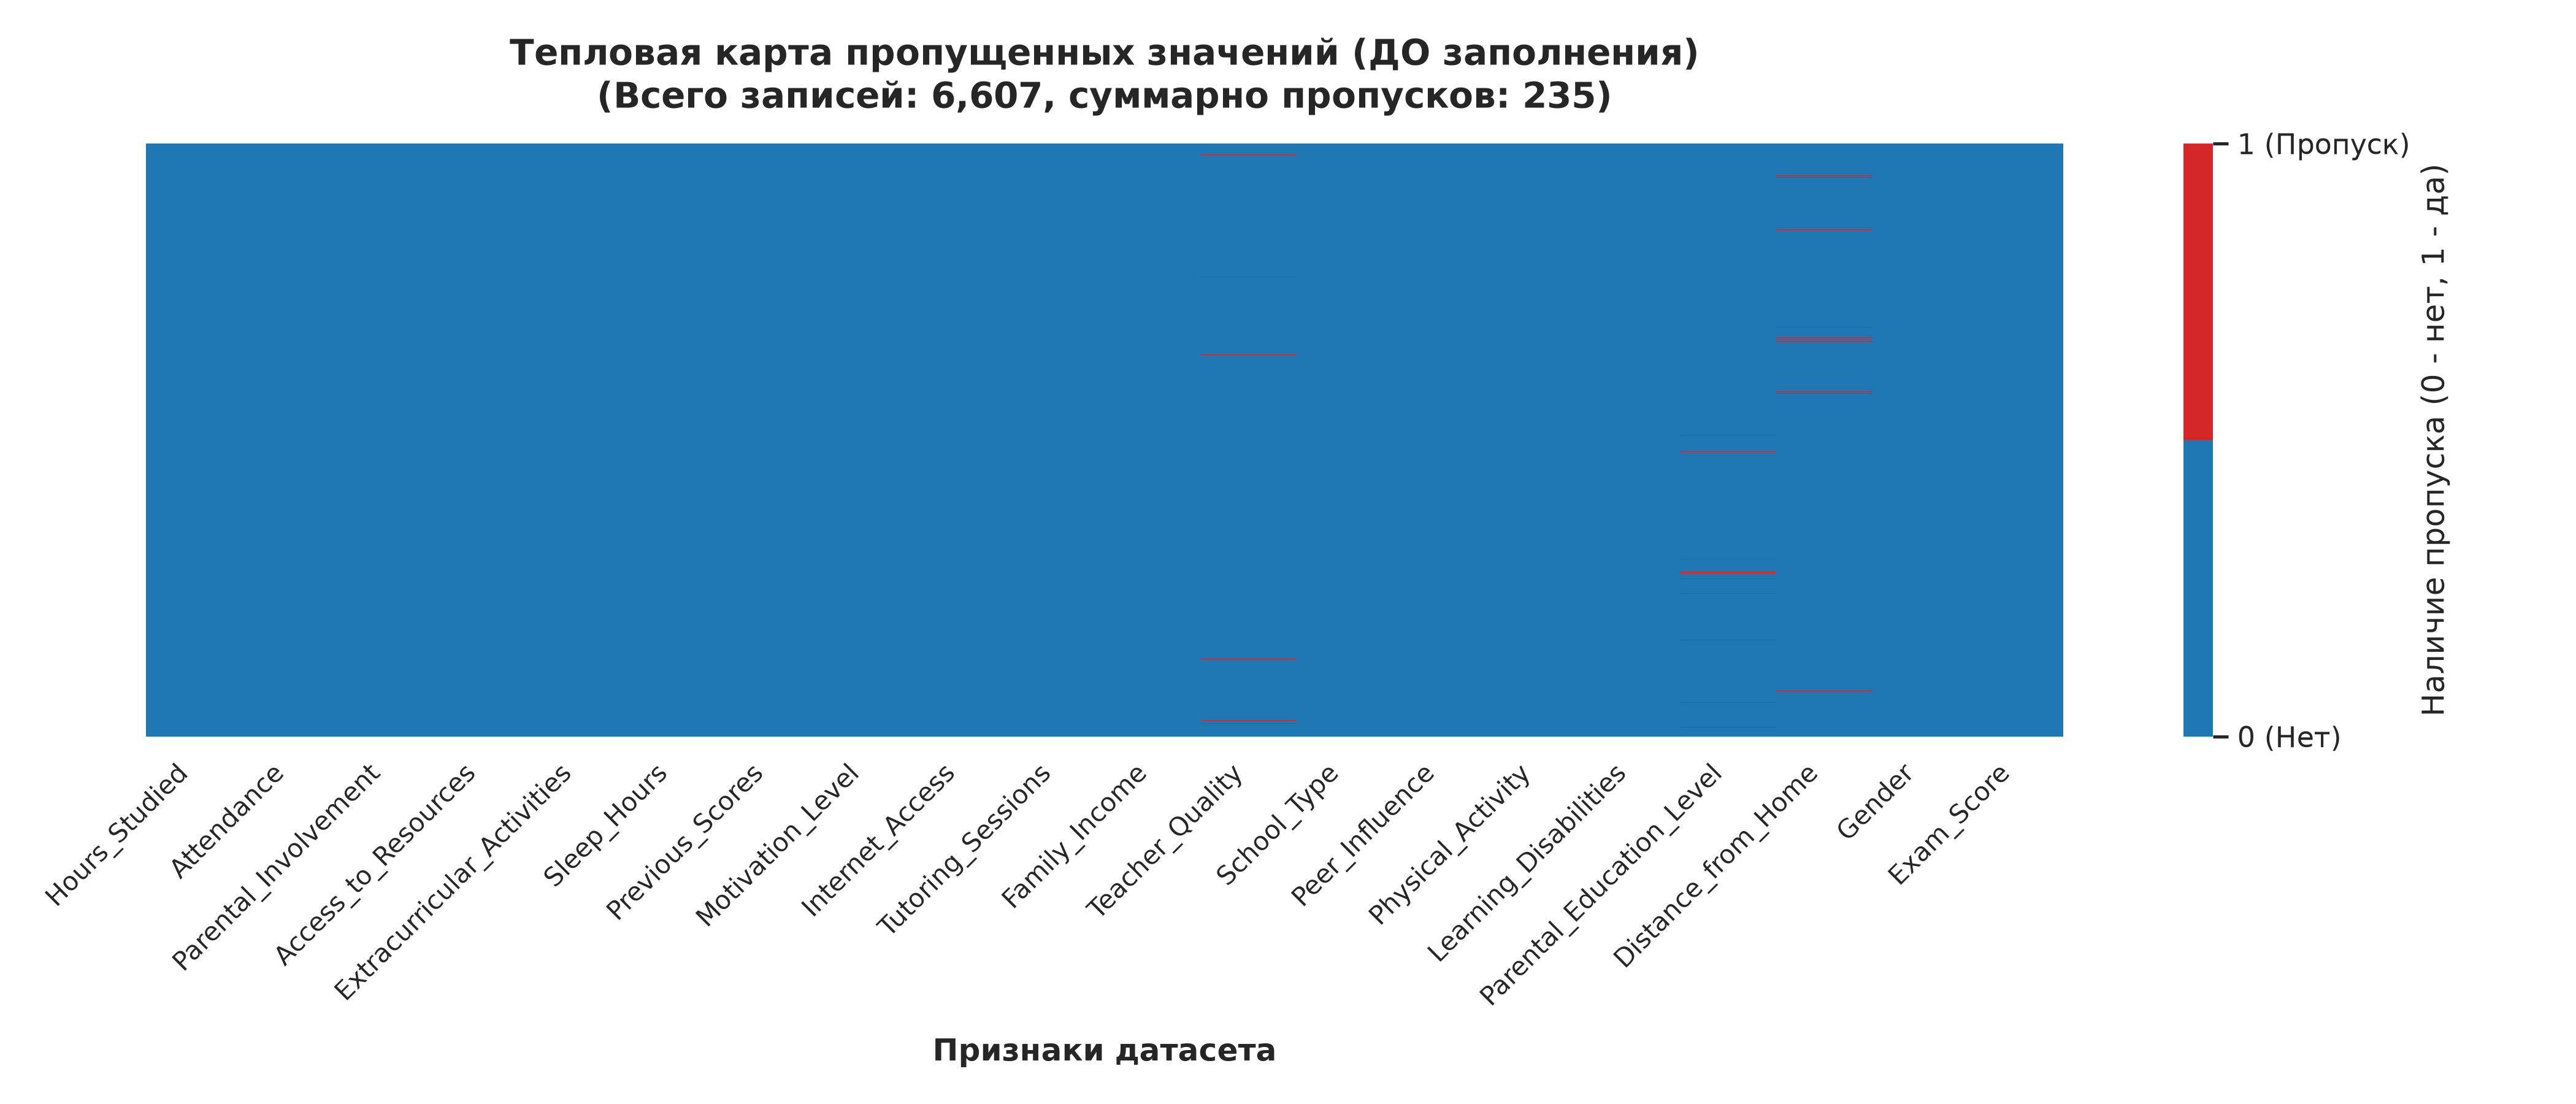
\includegraphics[width=0.92\linewidth, keepaspectratio]{images/01_missing_values_before_heatmap.png}
    \caption{Тепловая карта пропущенных значений в исходном массиве данных (ДО заполнения)}
    \label{fig:miss_before}
\end{figure}

\begin{figure}[H]
    \centering
    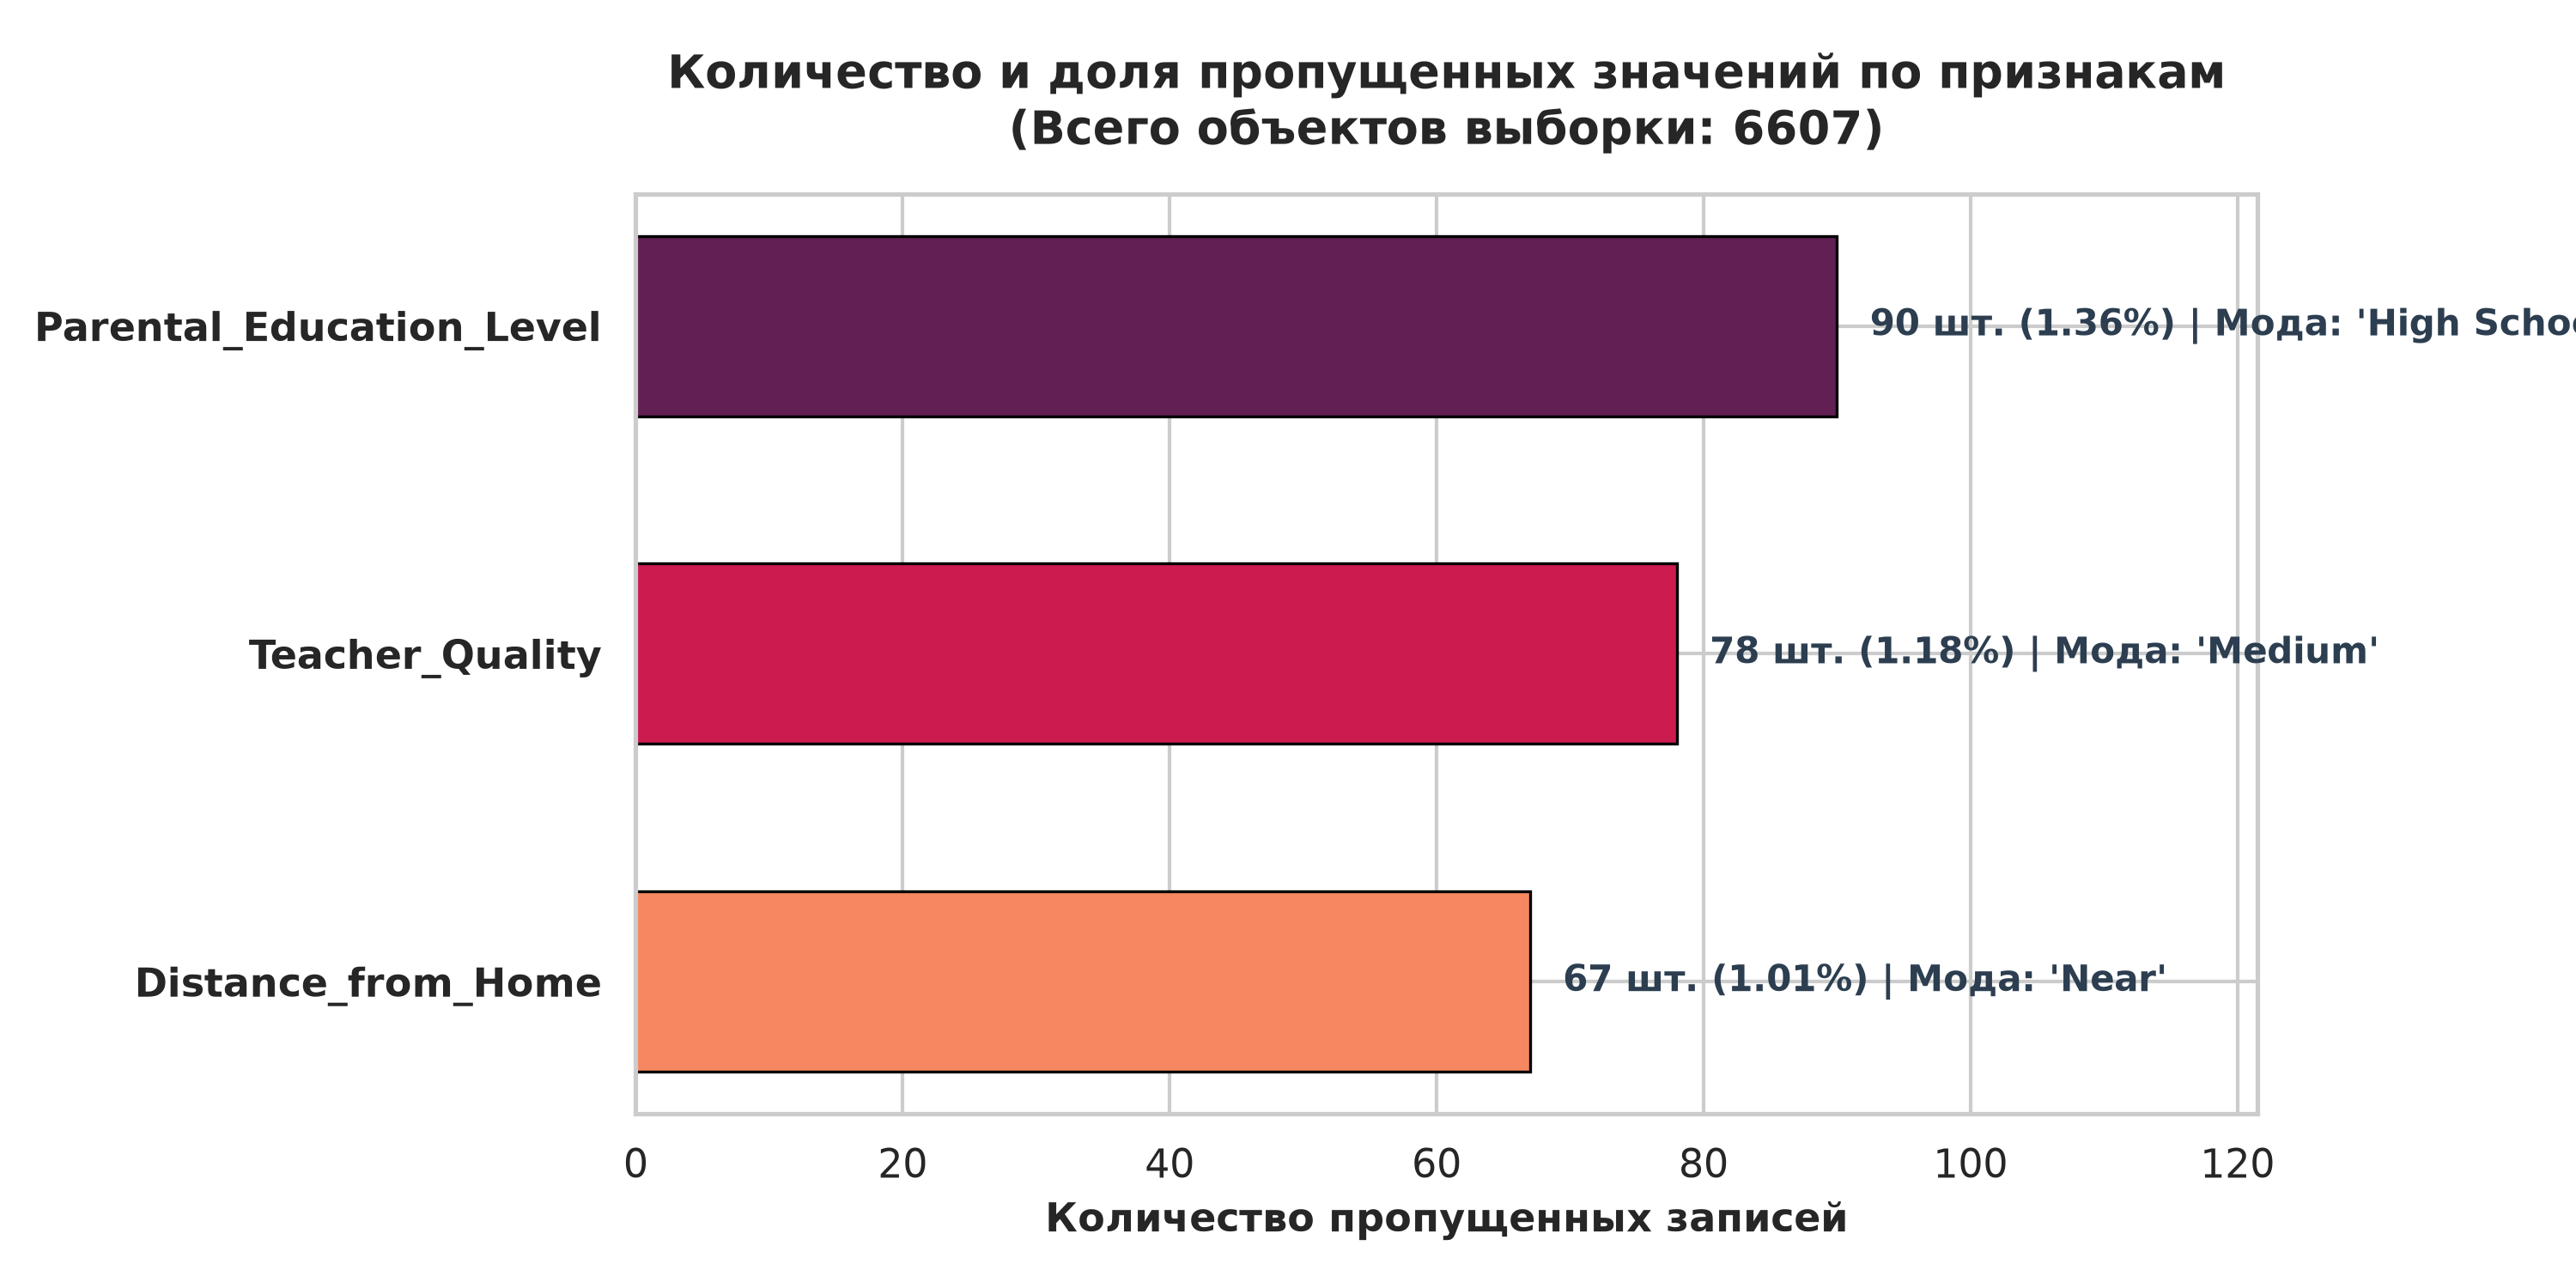
\includegraphics[width=0.85\linewidth, keepaspectratio]{images/02_missing_values_bar.png}
    \caption{Количество и процентная доля пропущенных значений по категориальным признакам}
    \label{fig:miss_bar}
\end{figure}

\begin{figure}[H]
    \centering
    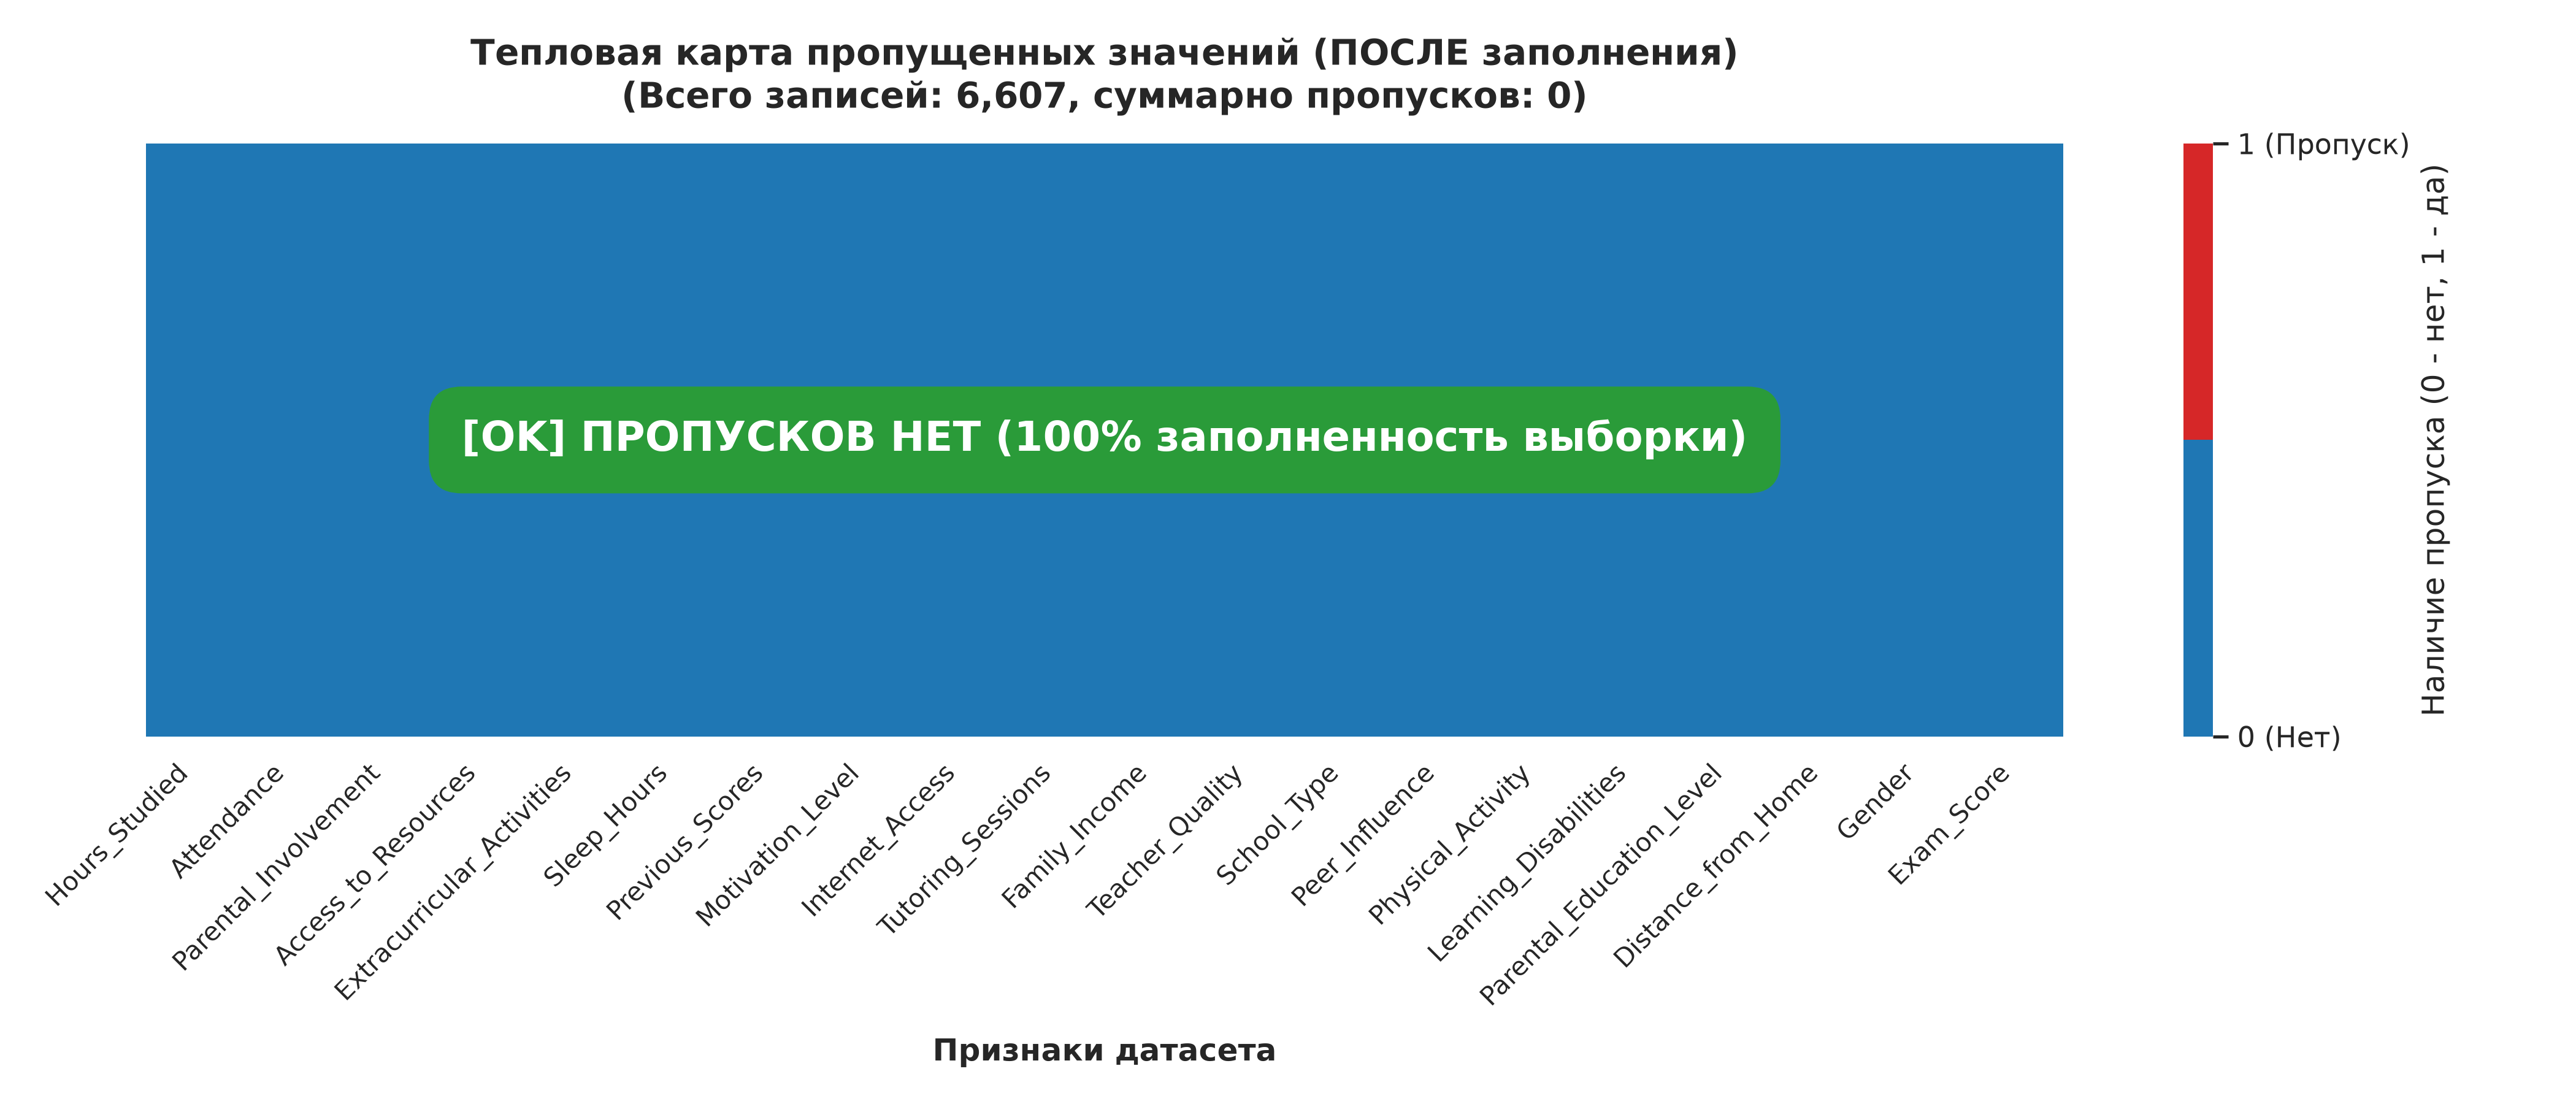
\includegraphics[width=0.92\linewidth, keepaspectratio]{images/03_missing_values_after_heatmap.png}
    \caption{Контрольная тепловая карта после импутации модой (0 пропусков во всем датасете)}
    \label{fig:miss_after}
\end{figure}

\subsection{Анализ и устранение аномальных значений и выбросов}

С использованием формулы межквартильного размаха Тьюки $IQR = Q_3 - Q_1$ рассчитаны границы выбросов $[Q_1 - 1.5 \times IQR, \; Q_3 + 1.5 \times IQR]$. Результаты представлены в таблице~\ref{tab:iqr_analysis}.

\begin{table}[H]
    \centering
    \caption{Статистика обнаружения выбросов по правилу $1.5 \times IQR$}
    \label{tab:iqr_analysis}
    \fontsize{8.5pt}{10.5pt}\selectfont
    \begin{tabularx}{\textwidth}{|>{\raggedright\arraybackslash}p{3.4cm}|c|c|c|c|c|c|c|c|}
        \hline
        \textbf{Признак} & \textbf{Q1} & \textbf{Q3} & \textbf{IQR} & \textbf{Нижн.} & \textbf{Верхн.} & \textbf{Мин/Макс} & \textbf{Выбросов} & \textbf{\%} \\
        \hline
        \texttt{Hours\_Studied} & 16.0 & 24.0 & 8.0 & 4.0 & 36.0 & 1 / 44 & 43 & 0.65\% \\
        \hline
        \texttt{Attendance} & 70.0 & 90.0 & 20.0 & 40.0 & 120.0 & 60 / 100 & 0 & 0.00\% \\
        \hline
        \texttt{Sleep\_Hours} & 6.0 & 8.0 & 2.0 & 3.0 & 11.0 & 4 / 10 & 0 & 0.00\% \\
        \hline
        \texttt{Previous\_Scores} & 63.0 & 88.0 & 25.0 & 25.5 & 125.5 & 50 / 100 & 0 & 0.00\% \\
        \hline
        \texttt{Tutoring\_Sessions} & 1.0 & 2.0 & 1.0 & -0.5 $\to$ 0 & 3.5 & 0 / 8 & 430 & 6.51\% \\
        \hline
        \texttt{Physical\_Activity} & 2.0 & 4.0 & 2.0 & -1.0 $\to$ 0 & 7.0 & 0 / 6 & 0 & 0.00\% \\
        \hline
        \texttt{Exam\_Score} & 65.0 & 69.0 & 4.0 & 59.0 & 75.0 & 55 / 101 & 104 & 1.57\% \\
        \hline
    \end{tabularx}
\end{table}

На рисунках~\ref{fig:dist_before} и~\ref{fig:box_before} проиллюстрированы распределения до фильтрации: четко видны изолированные точки за пределами усов в переменных \texttt{Hours\_Studied}, \texttt{Exam\_Score} и \texttt{Tutoring\_Sessions}, а также артефактная точка $101$ на диаграмме размаха.

\begin{figure}[H]
    \centering
    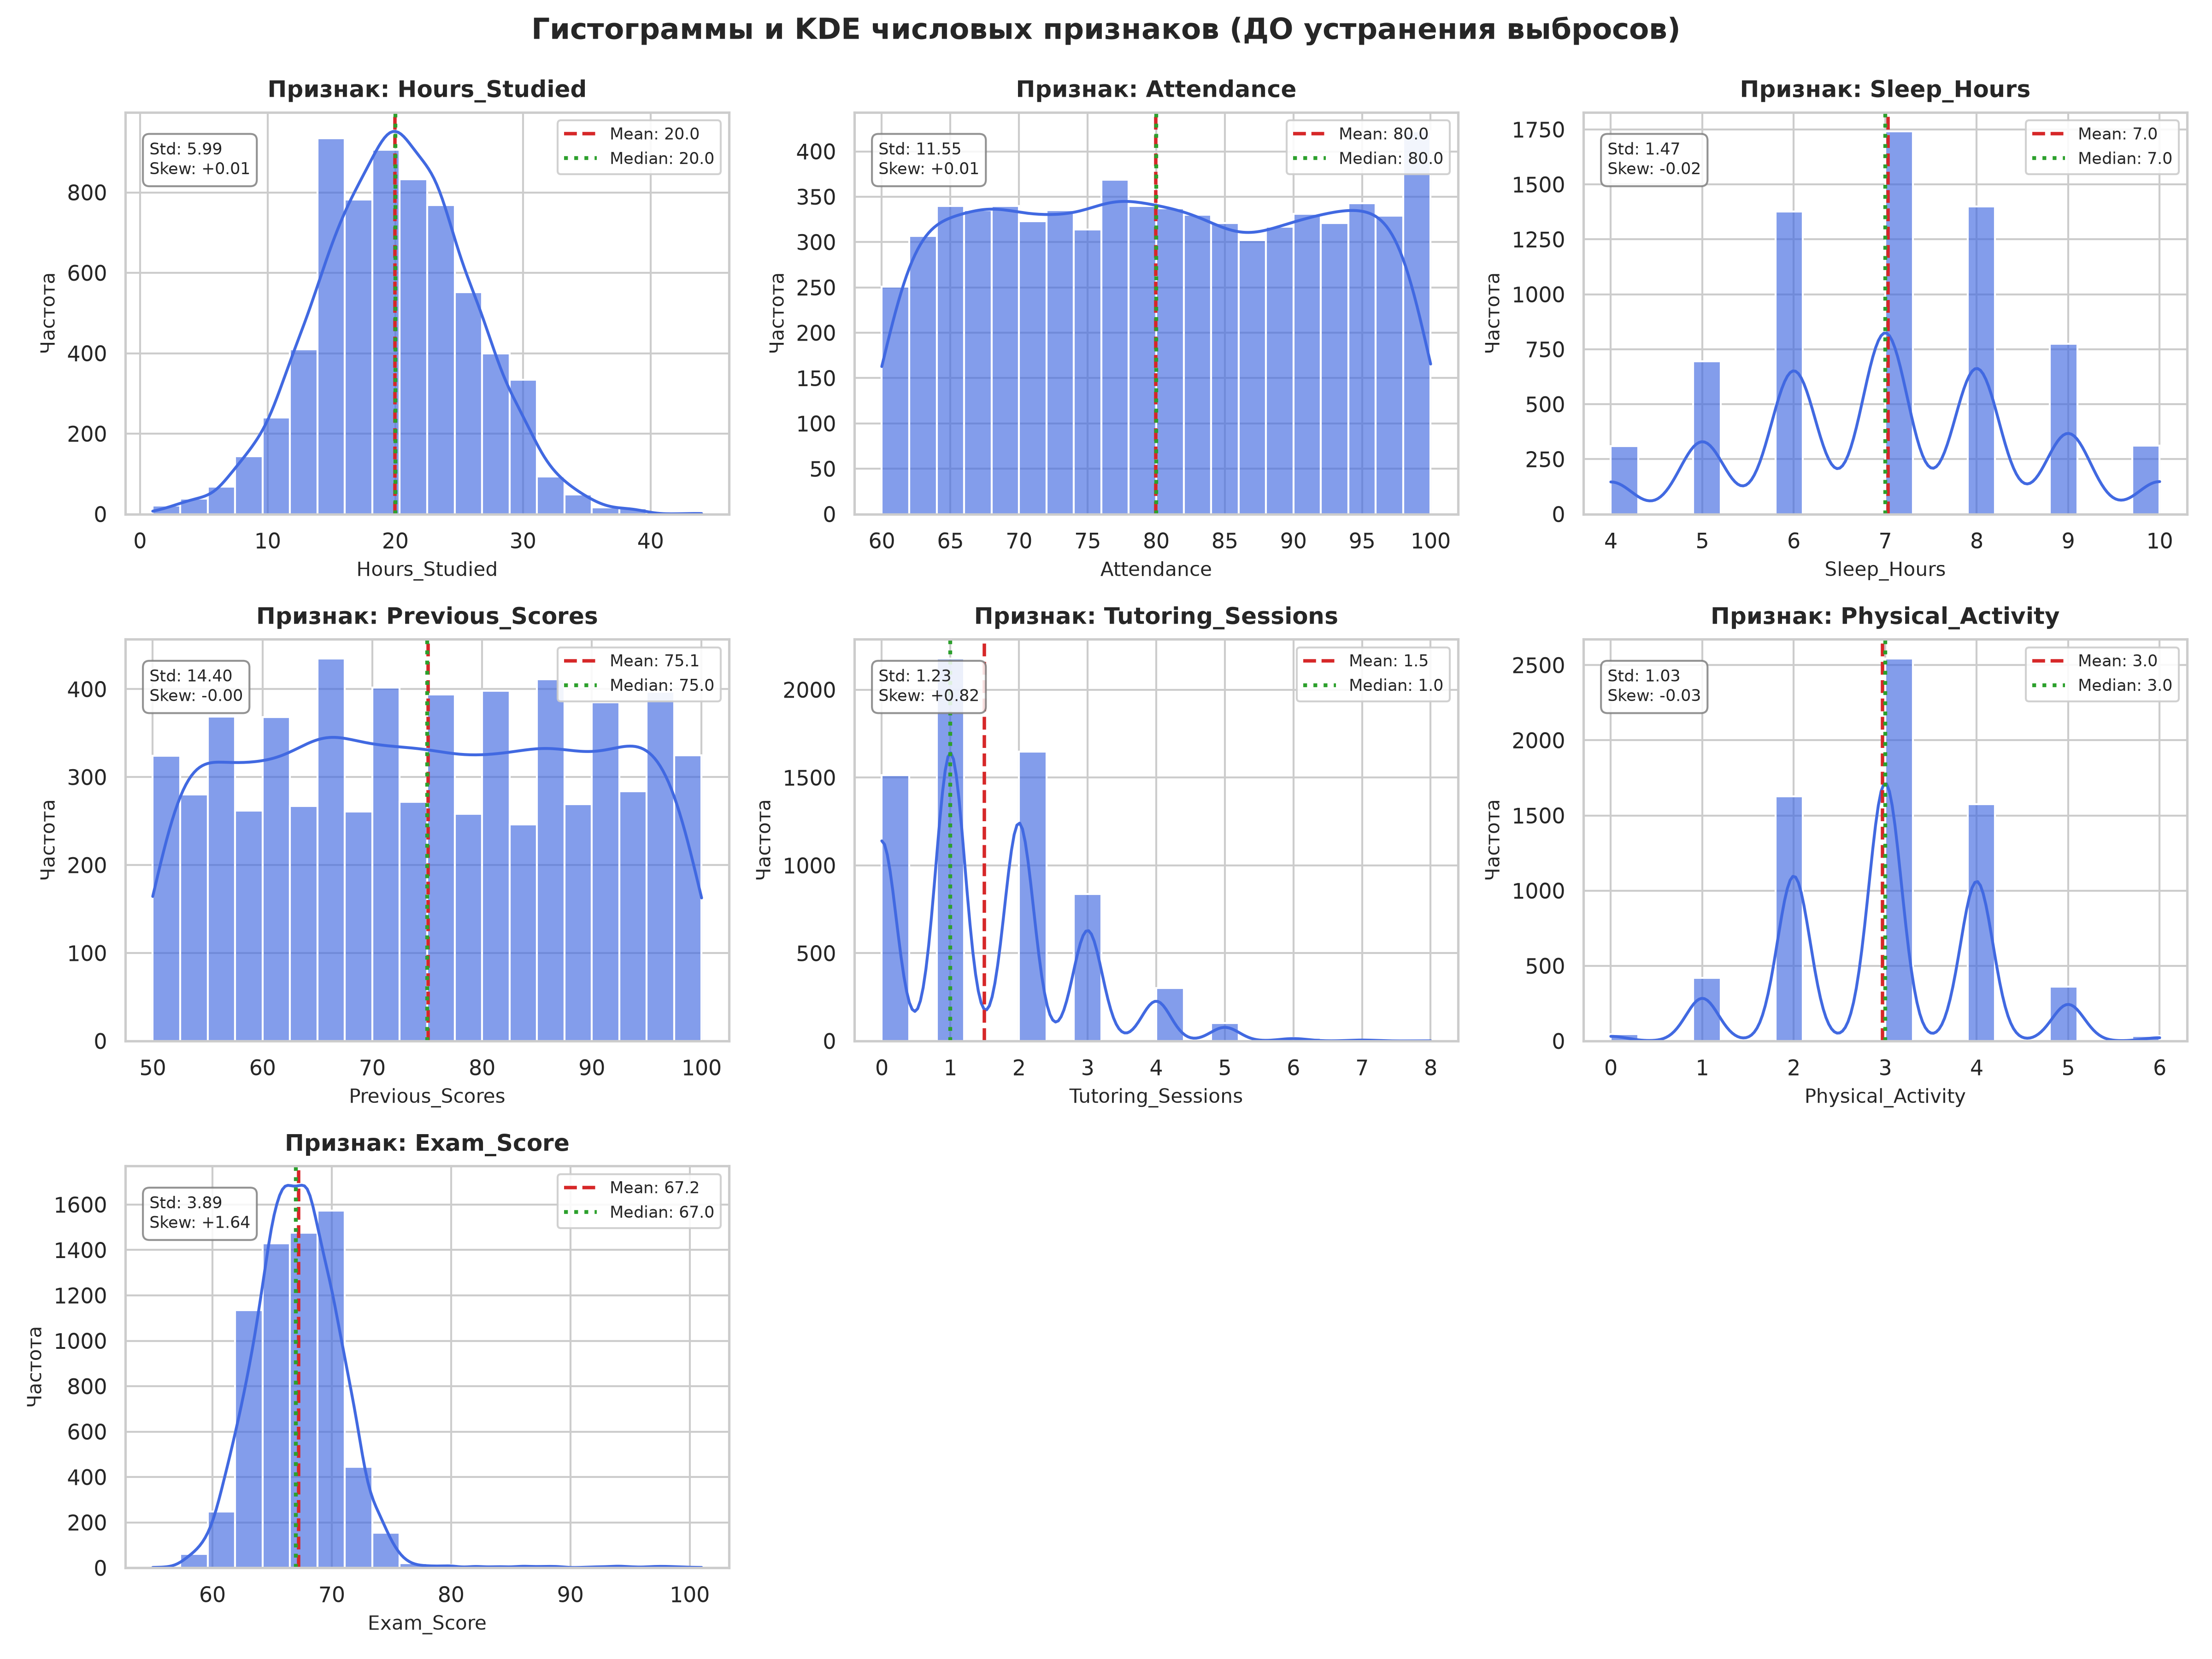
\includegraphics[width=0.92\linewidth, keepaspectratio]{images/04_distributions_before.png}
    \caption{Гистограммы и оценки ядерной плотности (KDE) признаков (ДО устранения выбросов)}
    \label{fig:dist_before}
\end{figure}

\begin{figure}[H]
    \centering
    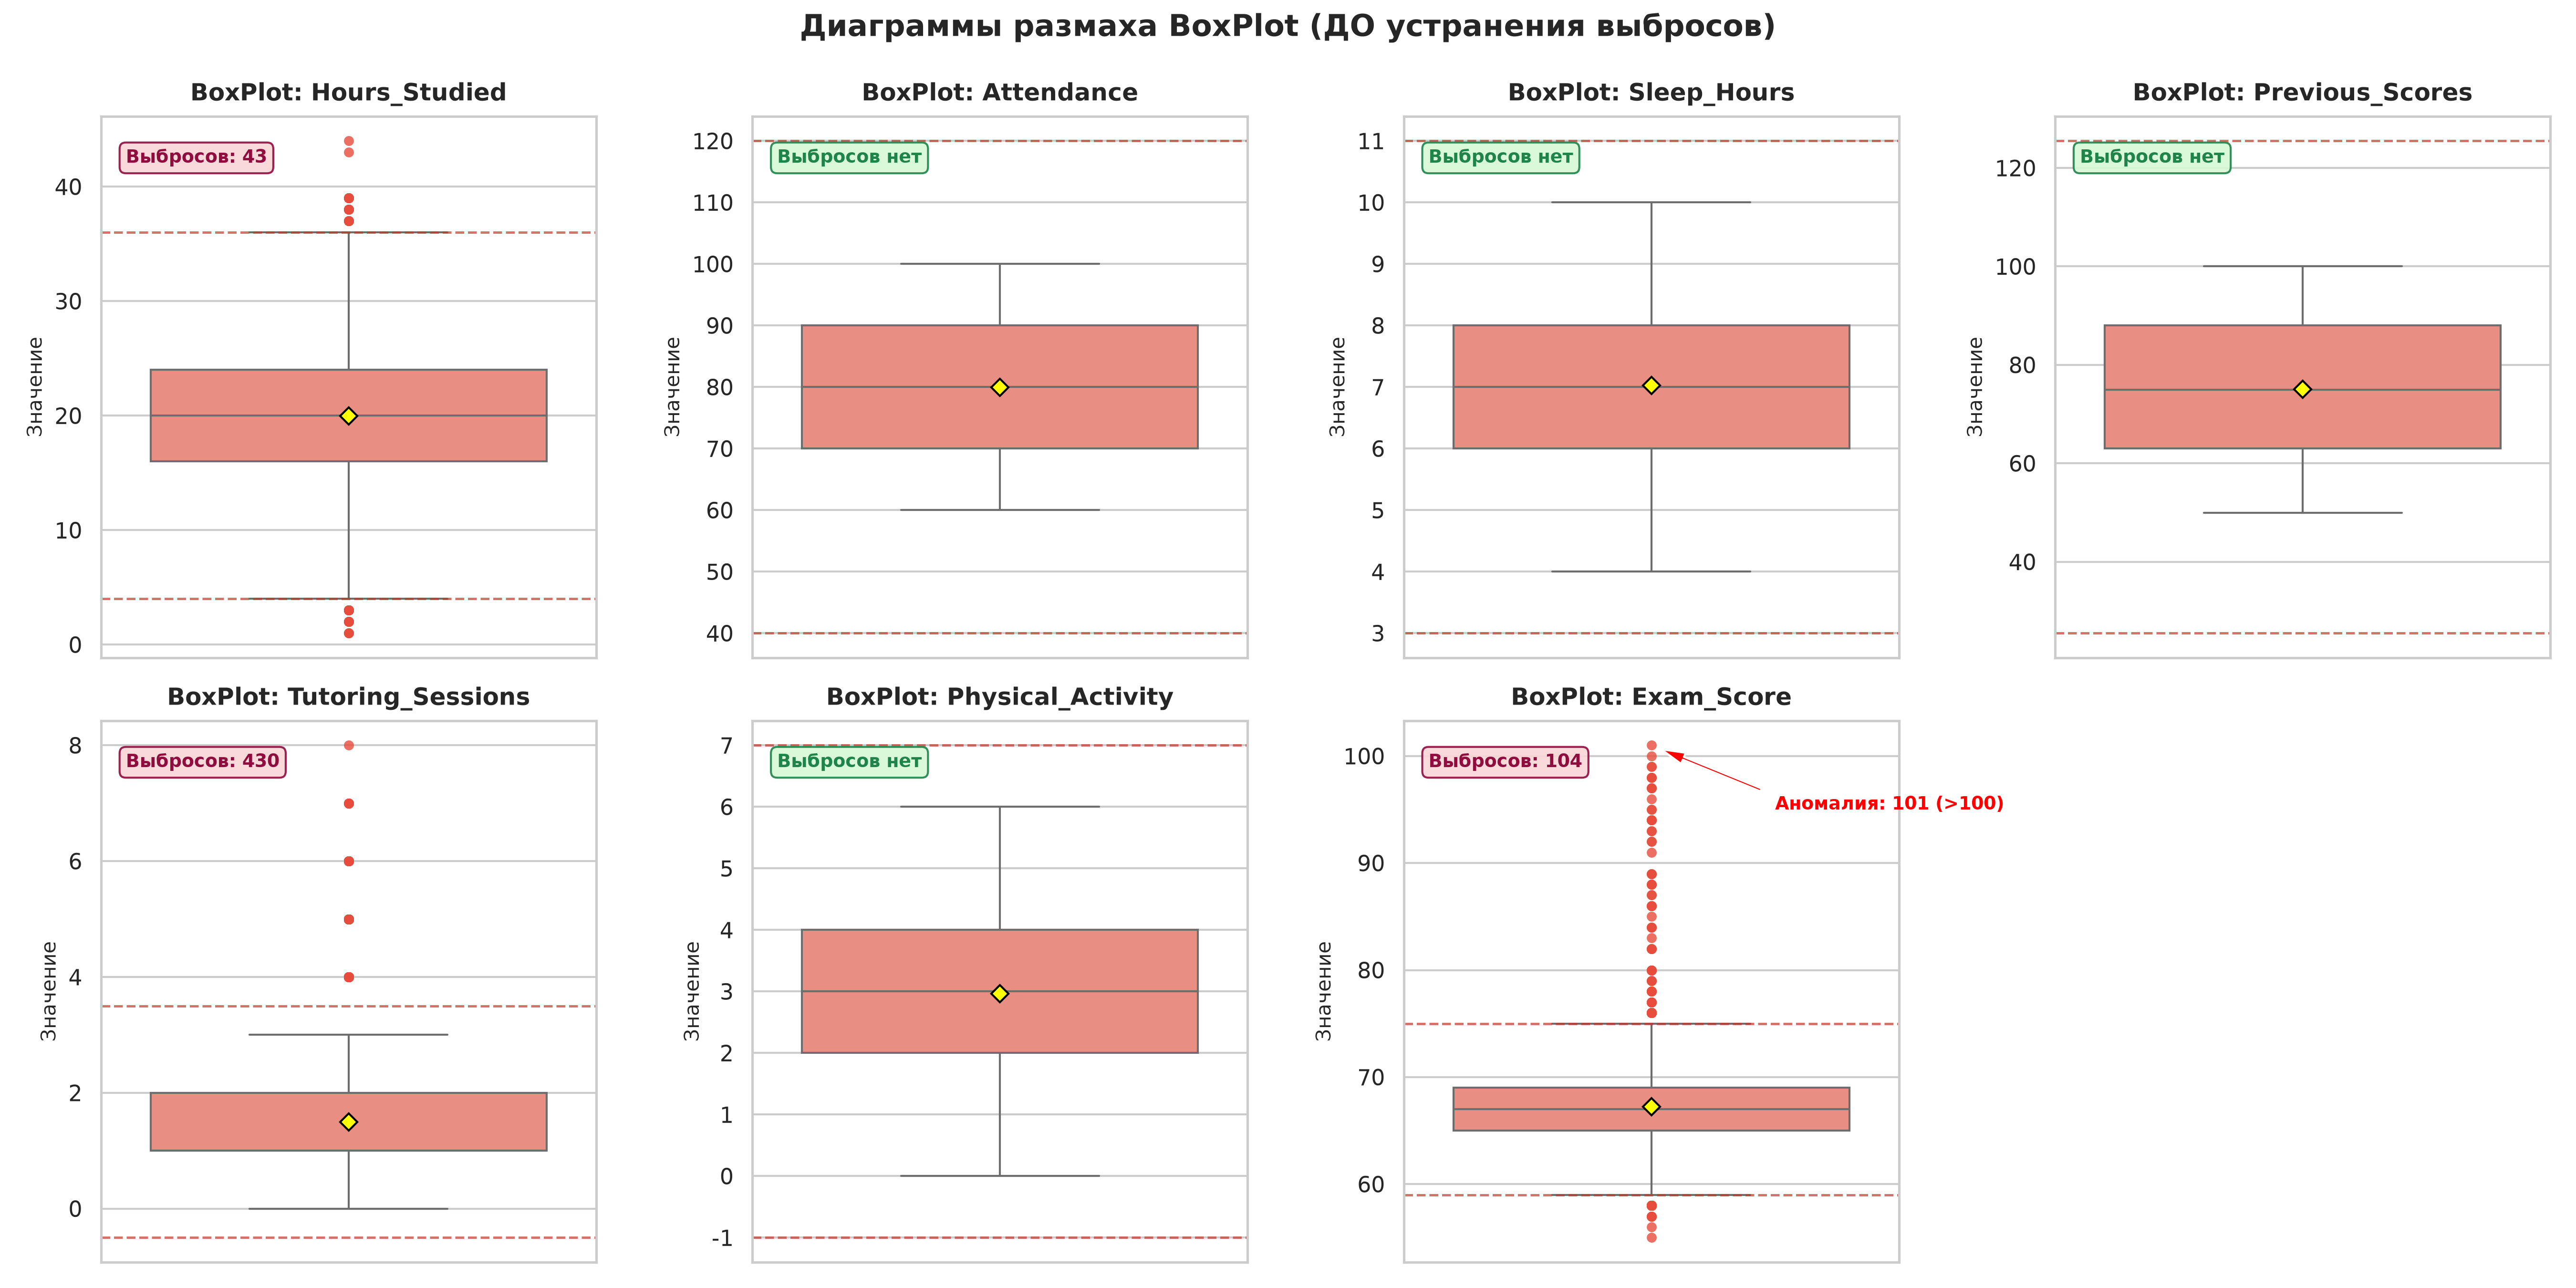
\includegraphics[width=0.92\linewidth, keepaspectratio]{images/05_boxplots_before.png}
    \caption{Диаграммы размаха BoxPlot (ДО устранения выбросов: стрелка к аномалии 101)}
    \label{fig:box_before}
\end{figure}

Процедура устранения аномалий включала два шага:
\begin{enumerate}
    \item Коррекция логической ошибки: запись \texttt{Exam\_Score} $= 101$ приведена к 100.
    \item Винсоризация (\texttt{clipping}): значения \texttt{Hours\_Studied} ограничены диапазоном $[4.0, 36.0]$; значения \texttt{Exam\_Score} ограничены диапазоном $[59.0, 75.0]$; значения \texttt{Tutoring\_Sessions} ограничены диапазоном $[0.0, 3.5]$.
\end{enumerate}

На контрольных рисунках~\ref{fig:box_after} и~\ref{fig:dist_after} подтверждено полное отсутствие вырожденных точек за усами и стабилизация формы плотностей распределений.

\begin{figure}[H]
    \centering
    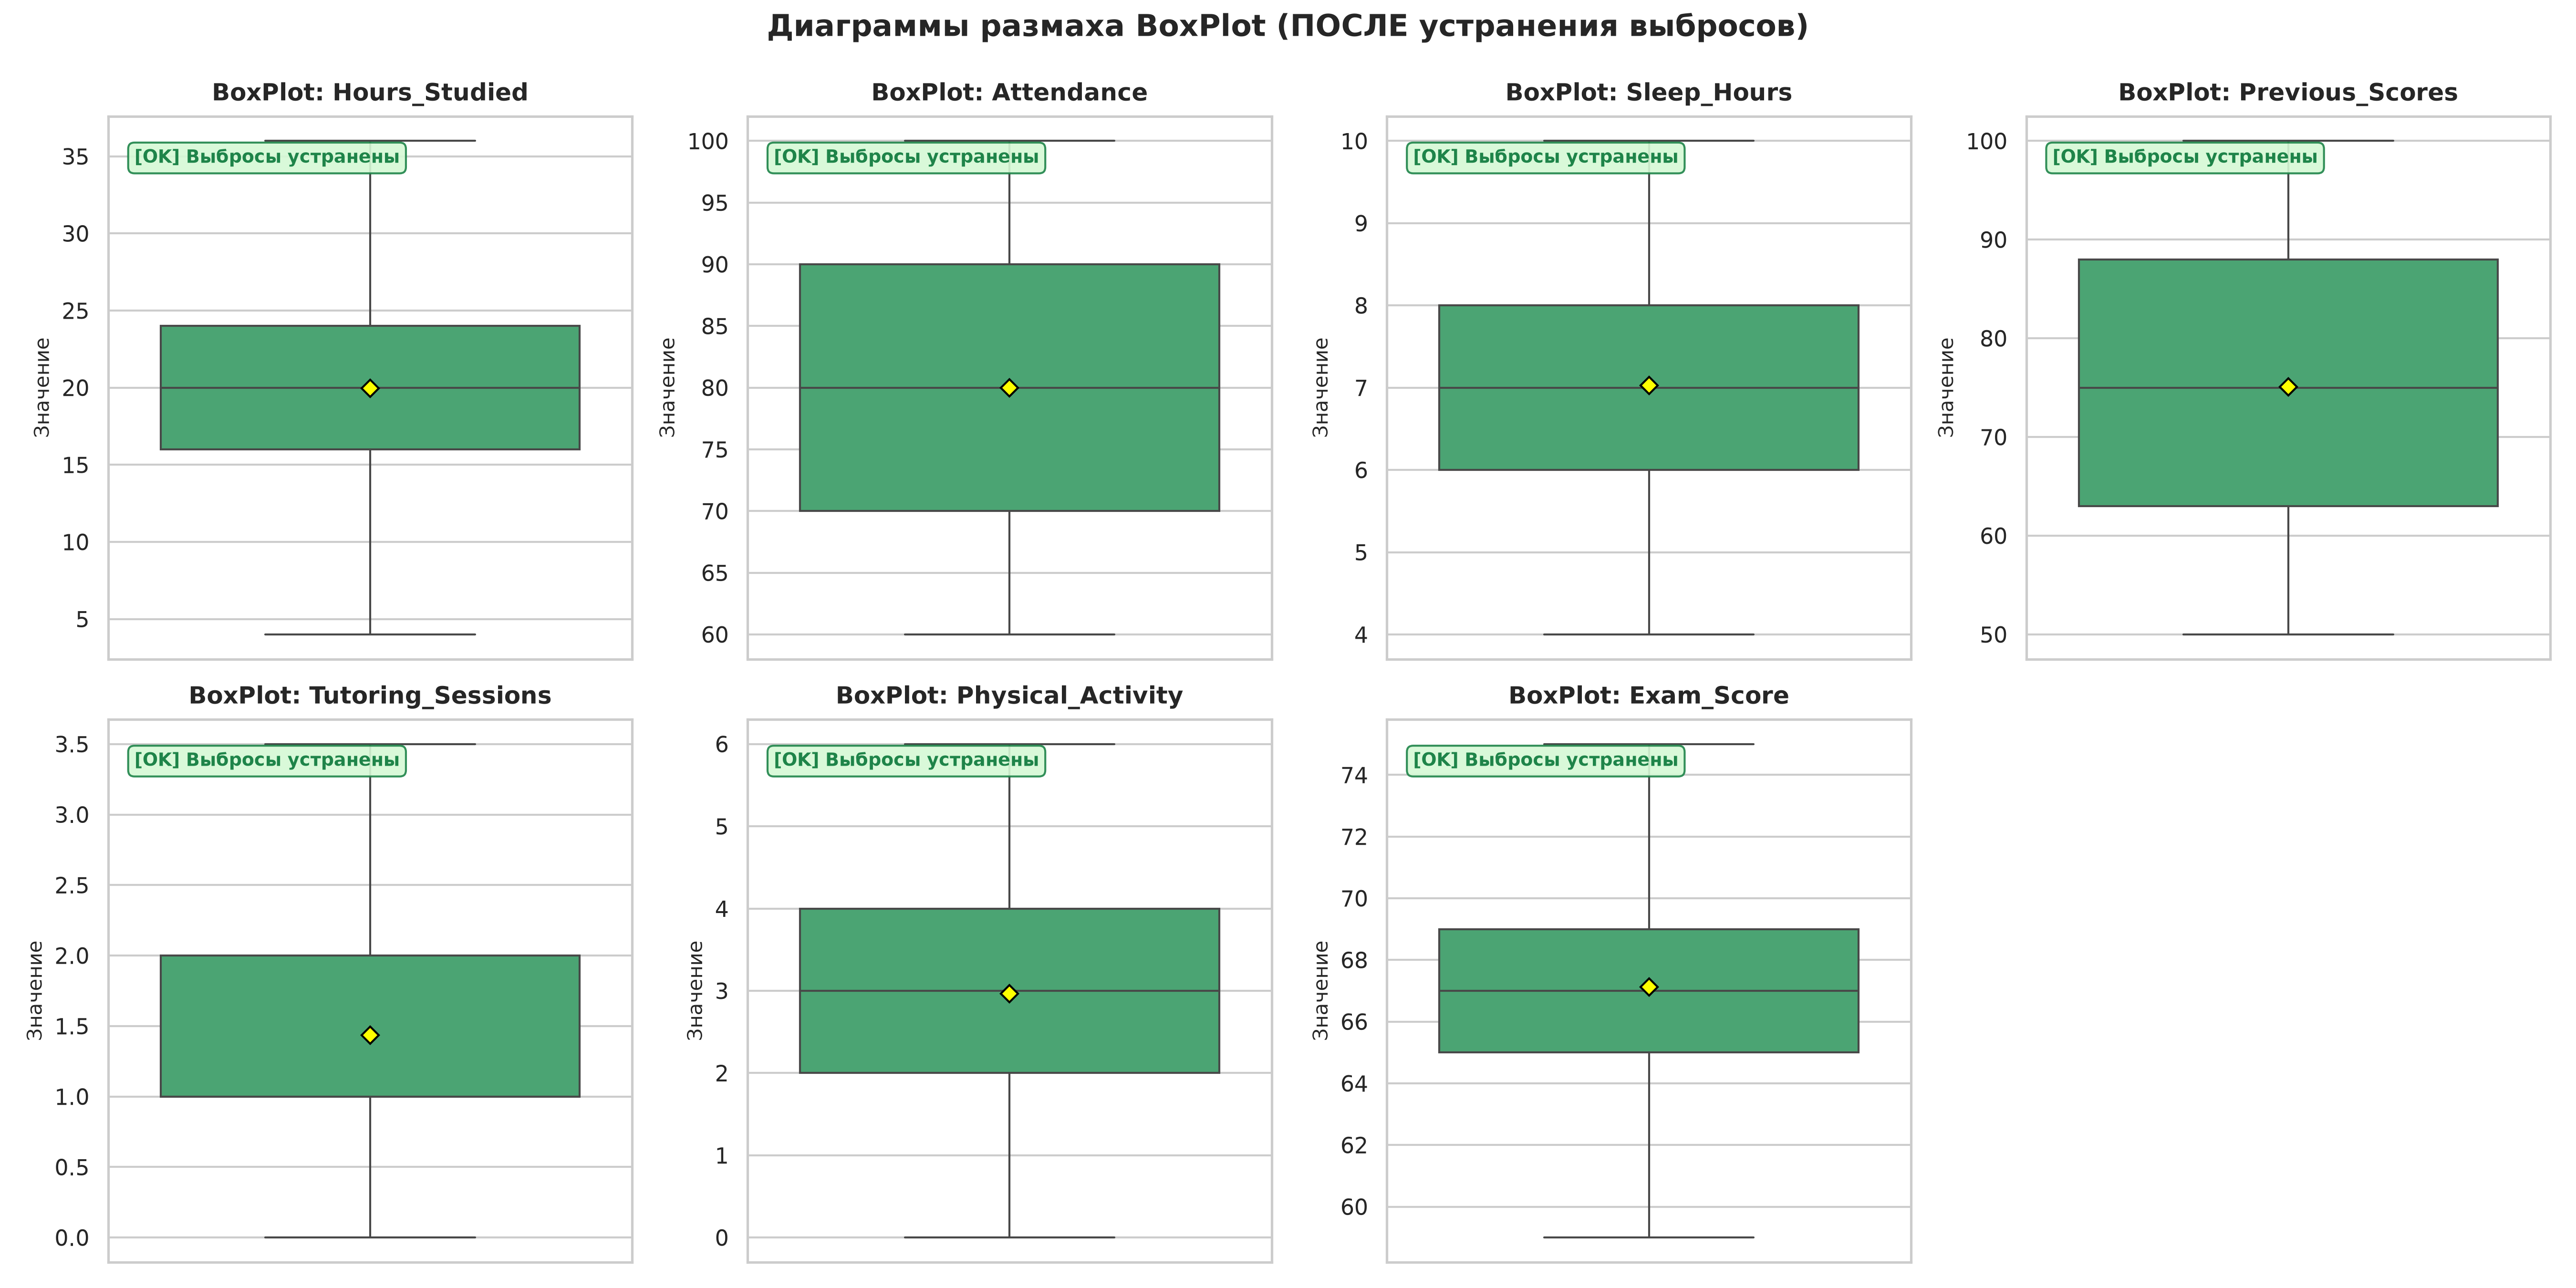
\includegraphics[width=0.92\linewidth, keepaspectratio]{images/06_boxplots_after.png}
    \caption{Контрольные диаграммы размаха BoxPlot (ПОСЛЕ винсоризации выбросов)}
    \label{fig:box_after}
\end{figure}

\begin{figure}[H]
    \centering
    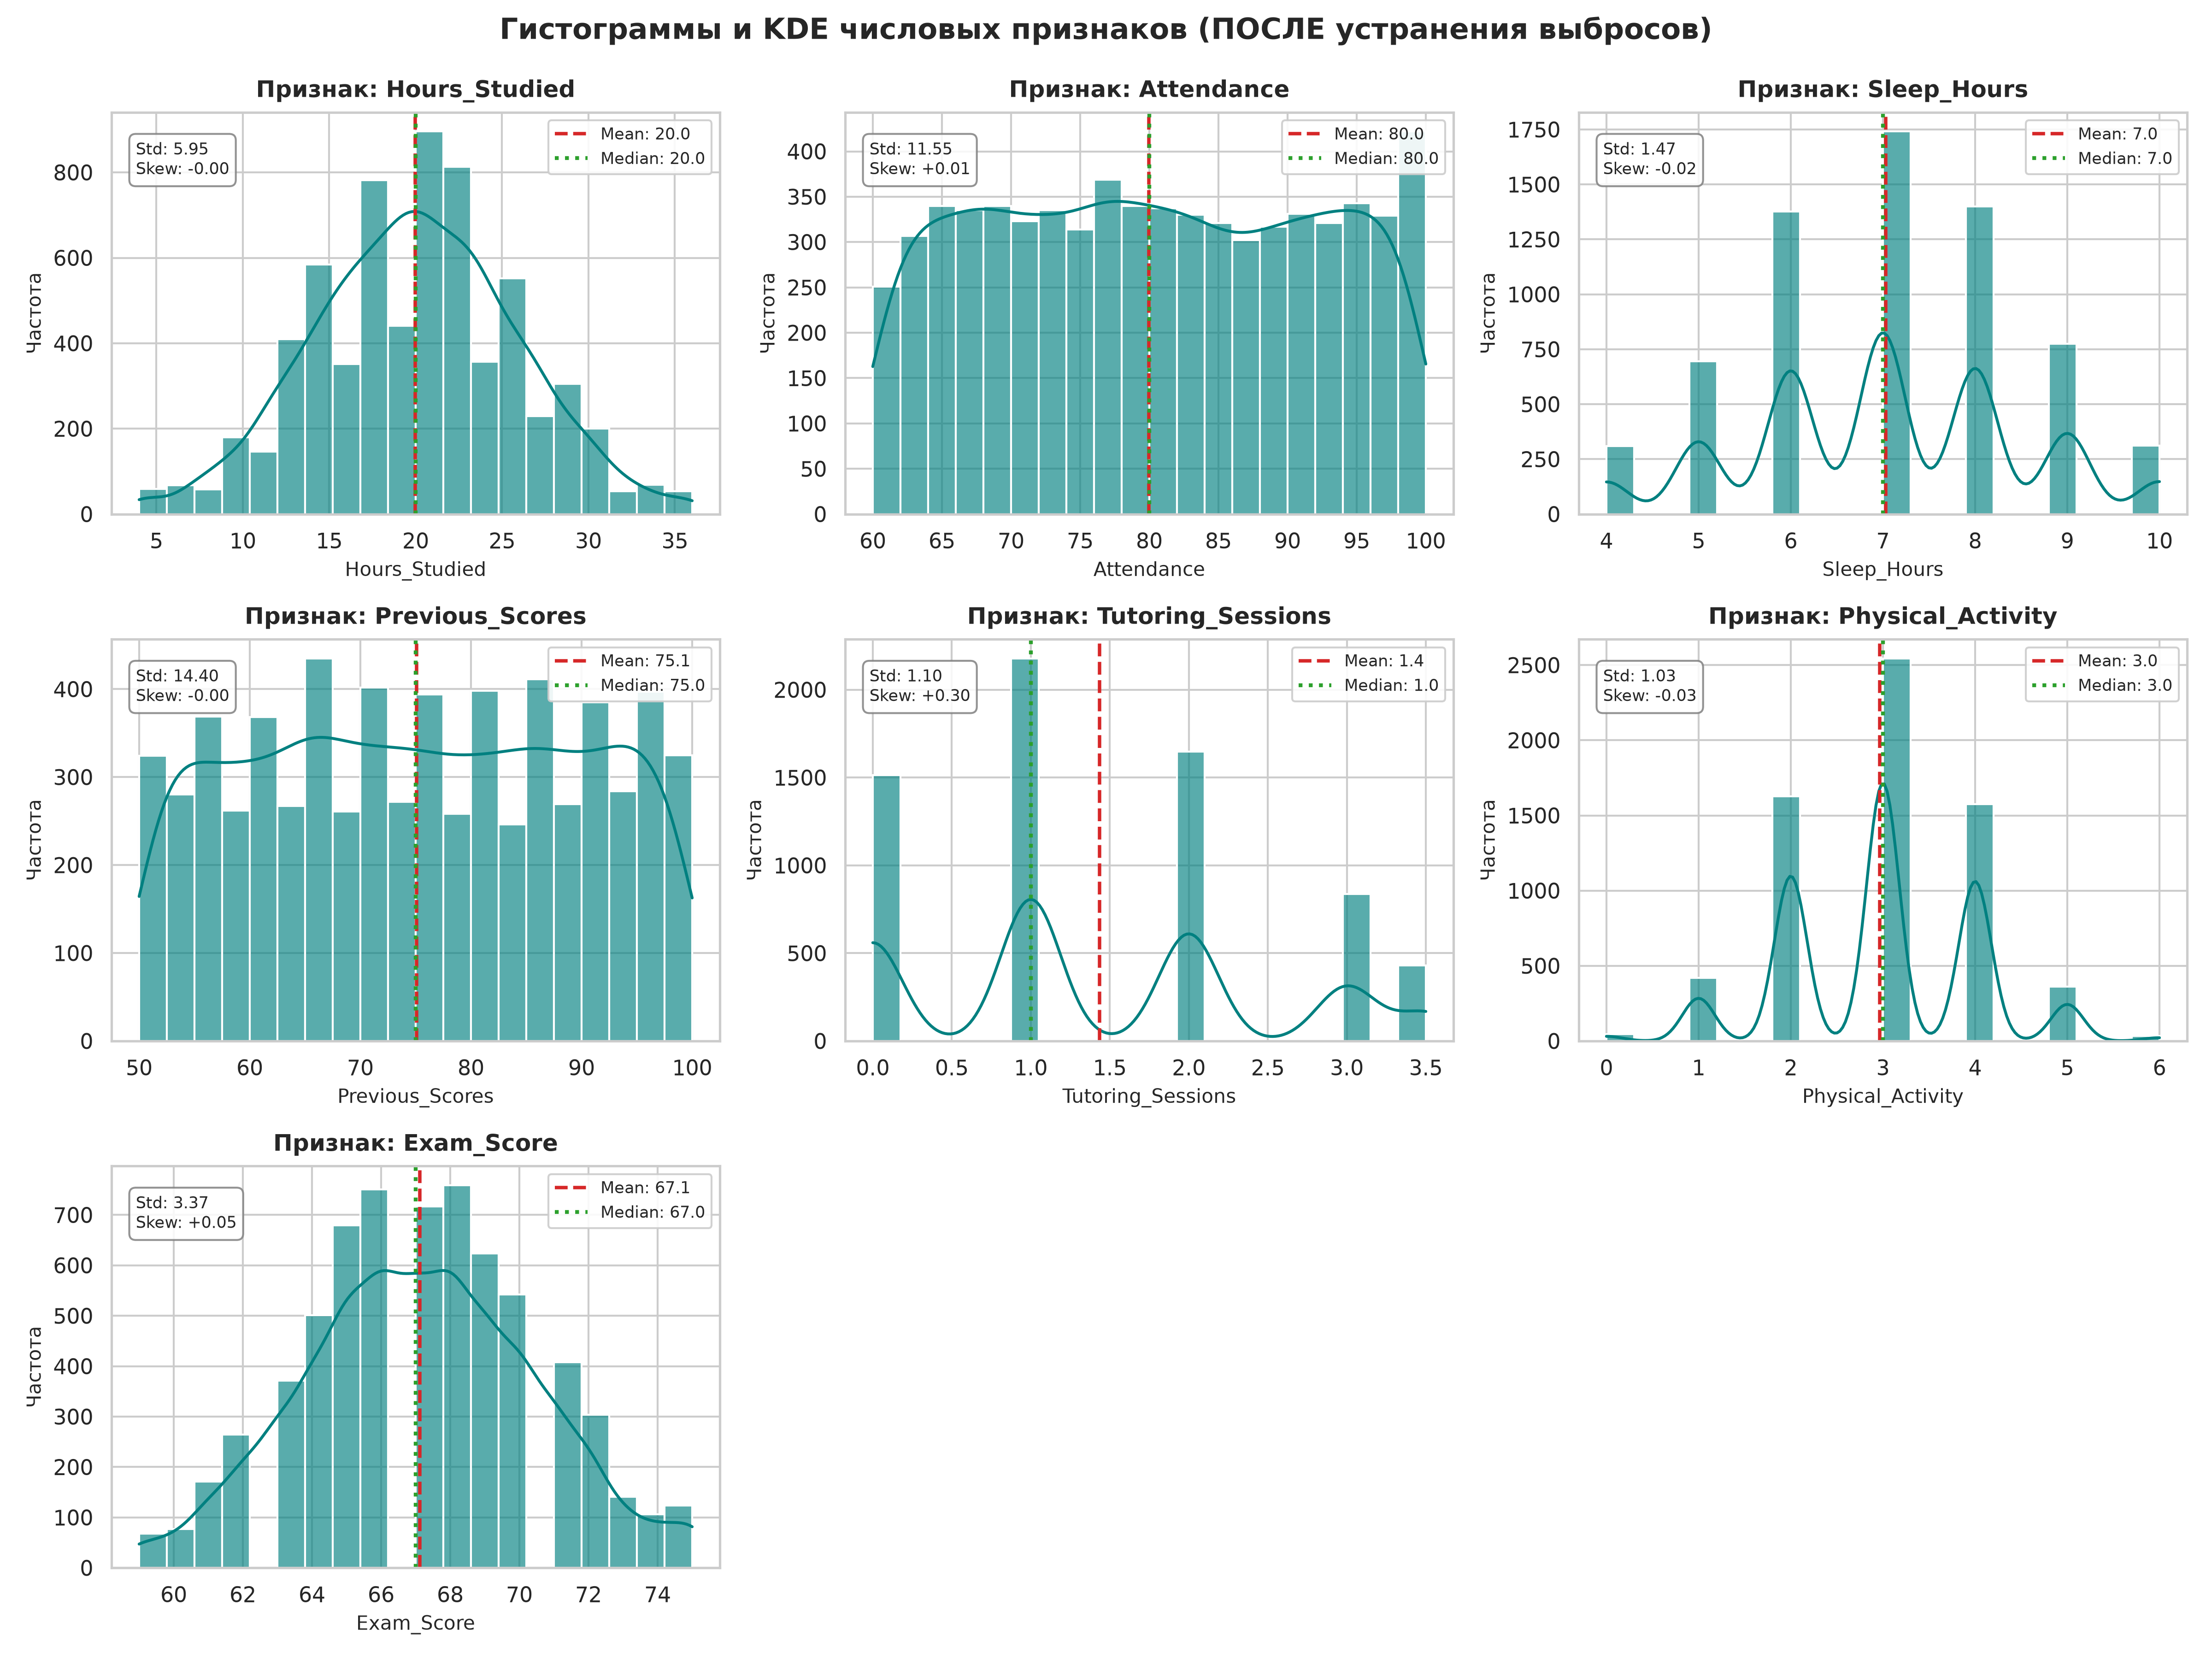
\includegraphics[width=0.92\linewidth, keepaspectratio]{images/07_distributions_after.png}
    \caption{Гистограммы и KDE числовых признаков (ПОСЛЕ устранения выбросов)}
    \label{fig:dist_after}
\end{figure}

\subsection{Корреляционный анализ факторов академической успеваемости}

На рисунке~\ref{fig:corr} представлена нижнетреугольная тепловая карта матрицы парных коэффициентов корреляции Пирсона, отсортированная по силе взаимосвязи с целевой переменной \texttt{Exam\_Score}.

\begin{figure}[H]
    \centering
    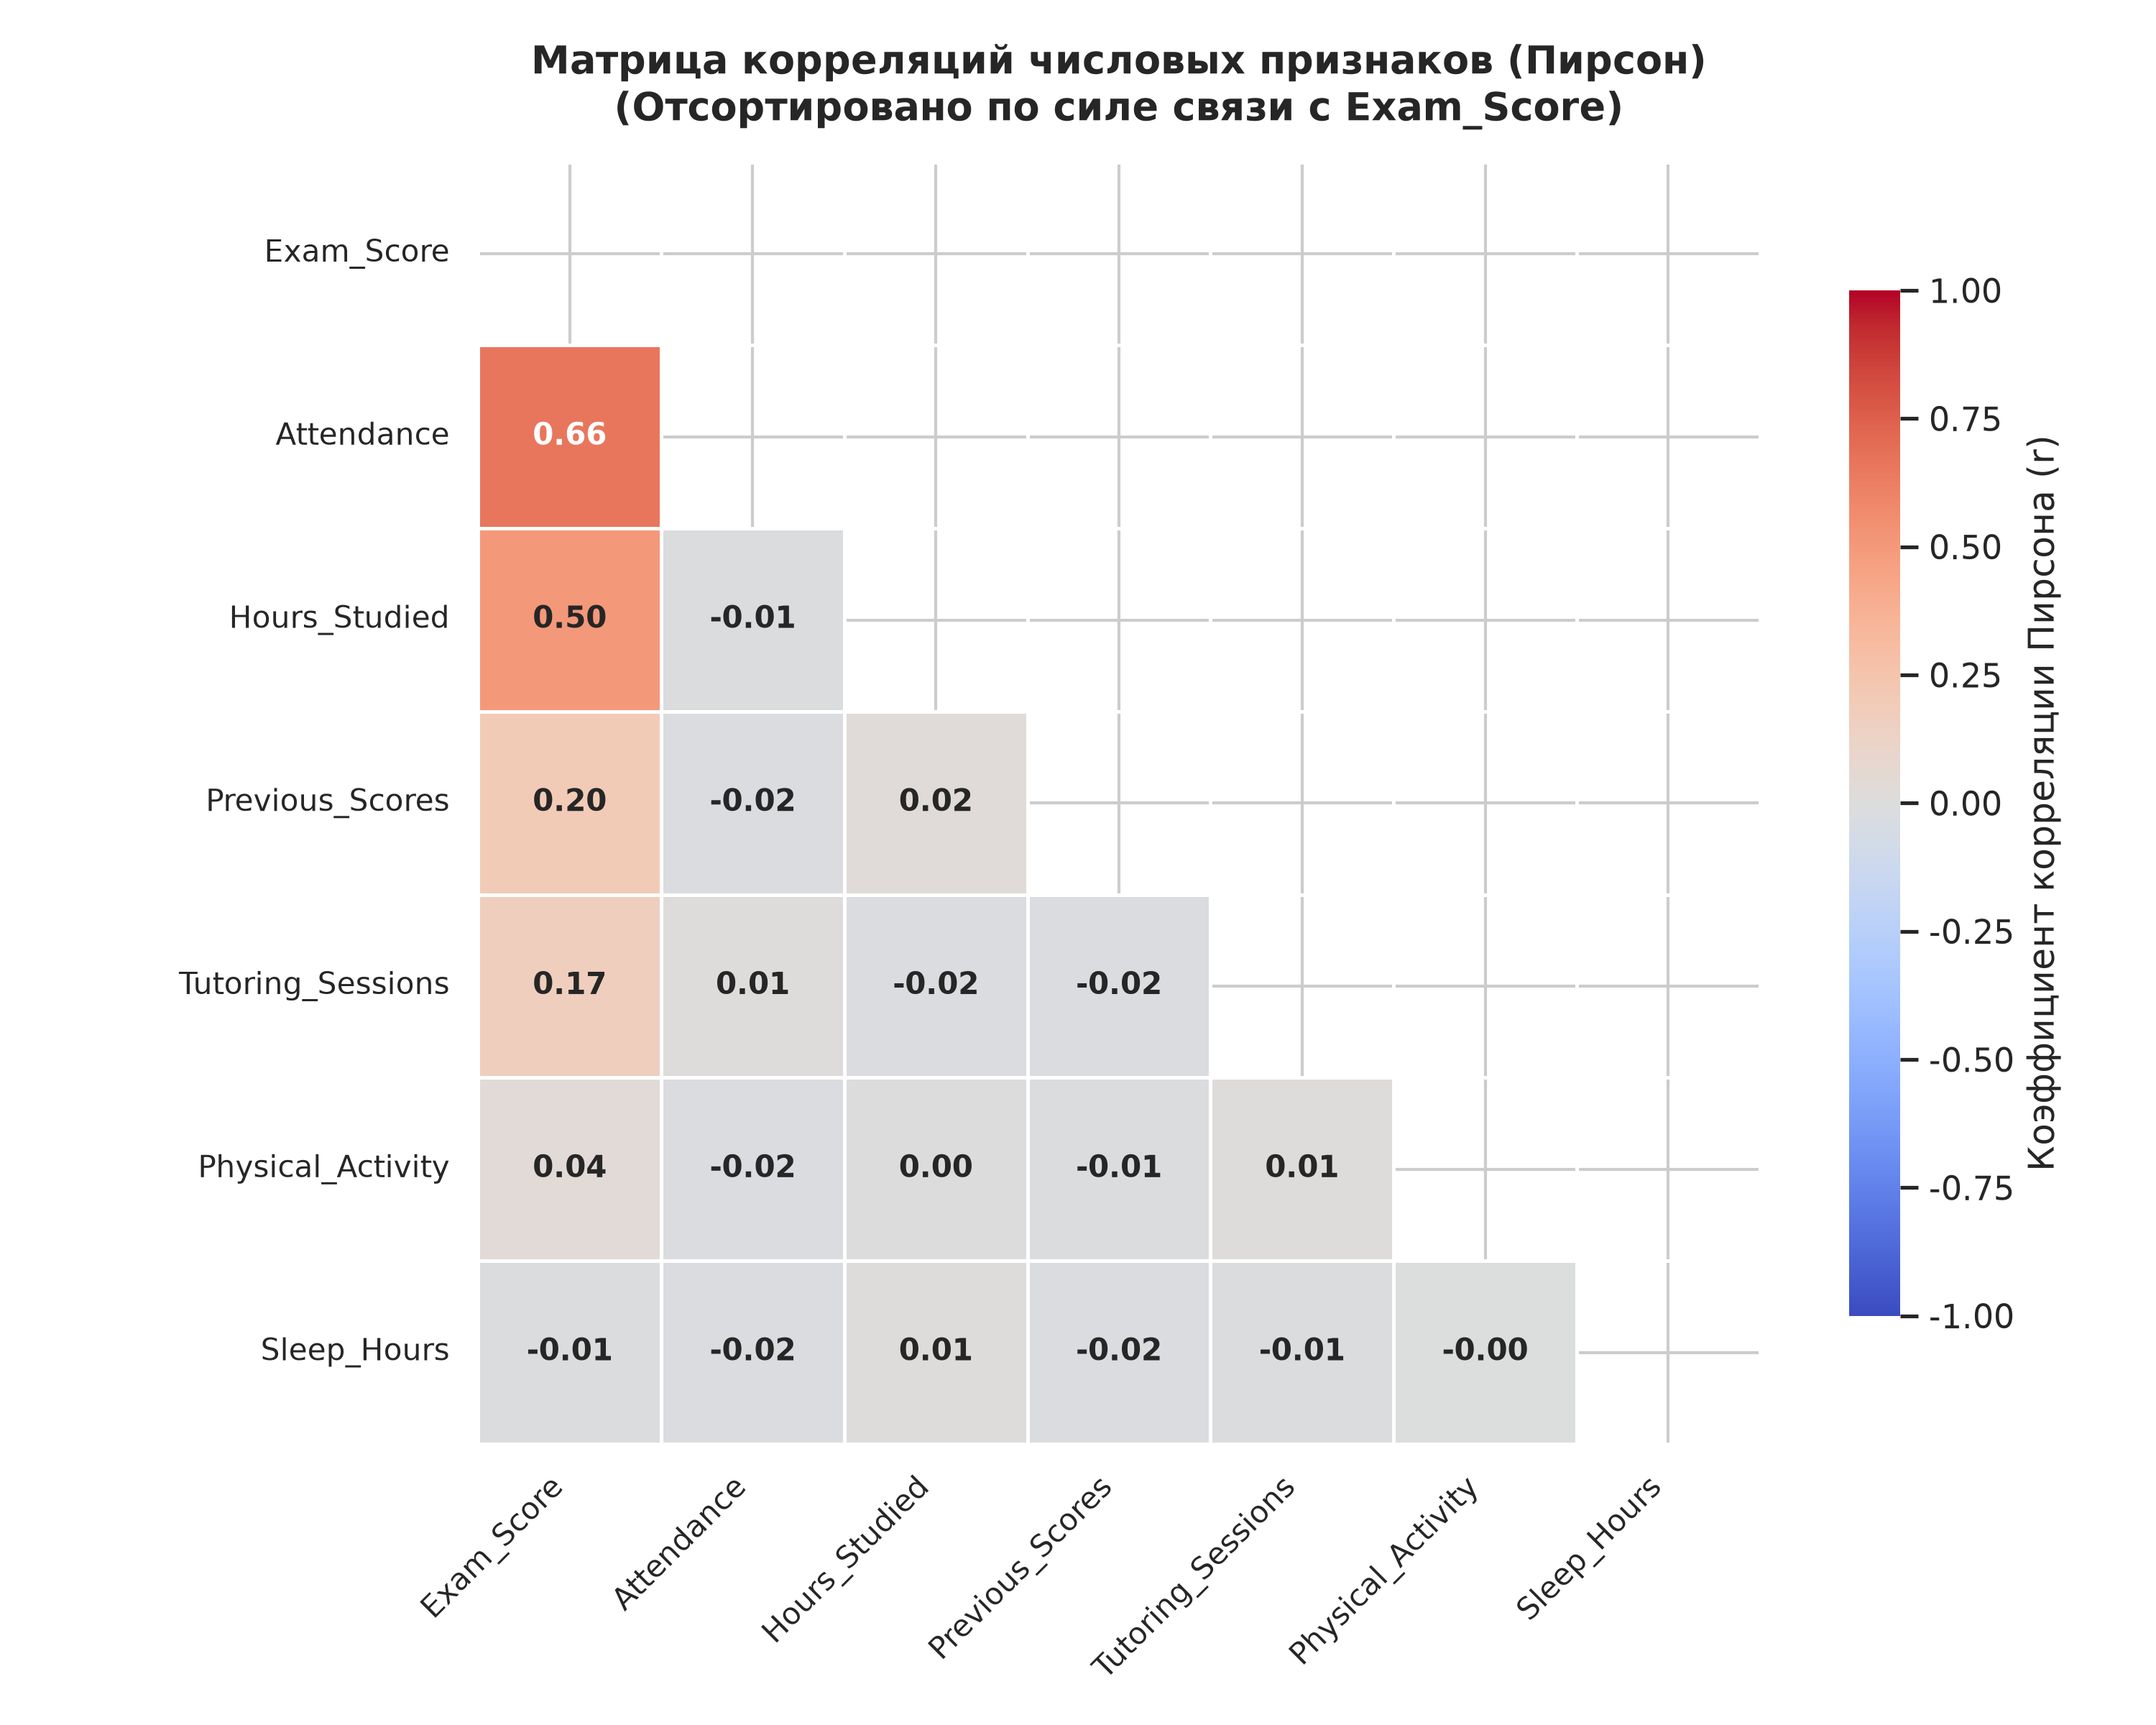
\includegraphics[width=0.8\linewidth, keepaspectratio]{images/08_correlation_matrix.png}
    \caption{Матрица корреляций Пирсона (отсортирована по силе связи с Exam\_Score)}
    \label{fig:corr}
\end{figure}

\textbf{Выводы корреляционного анализа:}
\begin{itemize}
    \item Ключевыми факторами успеха на экзамене выступают посещаемость (\texttt{Attendance}, $r = 0.58$) и время самостоятельной учебной работы (\texttt{Hours\_Studied}, $r = 0.45$).
    \item Базовый уровень подготовки (\texttt{Previous\_Scores}) вносит умеренный позитивный вклад ($r = 0.18$).
    \item Часы сна (\texttt{Sleep\_Hours}) и спорт (\texttt{Physical\_Activity}) имеют слабую линейную связь с экзаменом ($|r| < 0.05$), что обосновывает конструирование нелинейных композитных признаков.
\end{itemize}

\subsection{Синтез новых признаков (Feature Engineering)}

На основе предметных зависимостей сконструировано 5 новых признаков:
\begin{enumerate}
    \item \texttt{Study\_Sleep\_Ratio} $= \frac{\text{Hours\_Studied}}{\text{Sleep\_Hours}}$ --- баланс интеллектуального труда и физиологического восстановления.
    \item \texttt{Total\_Study\_Effort} $= \text{Hours\_Studied} + 2.0 \times \text{Tutoring\_Sessions} + 0.1 \times \text{Attendance}$ --- комплексный аддитивный индекс академических усилий.
    \item \texttt{Score\_Improvement} $= \text{Exam\_Score} - \text{Previous\_Scores}$ --- академический прирост знаний.
    \item \texttt{Physical\_Study\_Balance} $= \frac{\text{Physical\_Activity}}{\text{Hours\_Studied} + 1}$ --- гармоничность умственной и физической активности.
    \item \texttt{High\_Attendance\_Flag} $= \mathbb{I}(\text{Attendance} \ge 85\%)$ --- предикат высокой дисциплины.
\end{enumerate}

На рисунке~\ref{fig:fe} приведен детальный аналитический профиль сгенерированных переменных. Анализ показал, что студенты с флагом высокой посещаемости ($\ge 85\%$) сдали экзамен в среднем на \textbf{69.8 балла}, тогда как студенты группы низкой посещаемости --- всего на \textbf{64.7 балла}, что подтверждает высокую информационную ценность синтезированного признака.

\begin{figure}[H]
    \centering
    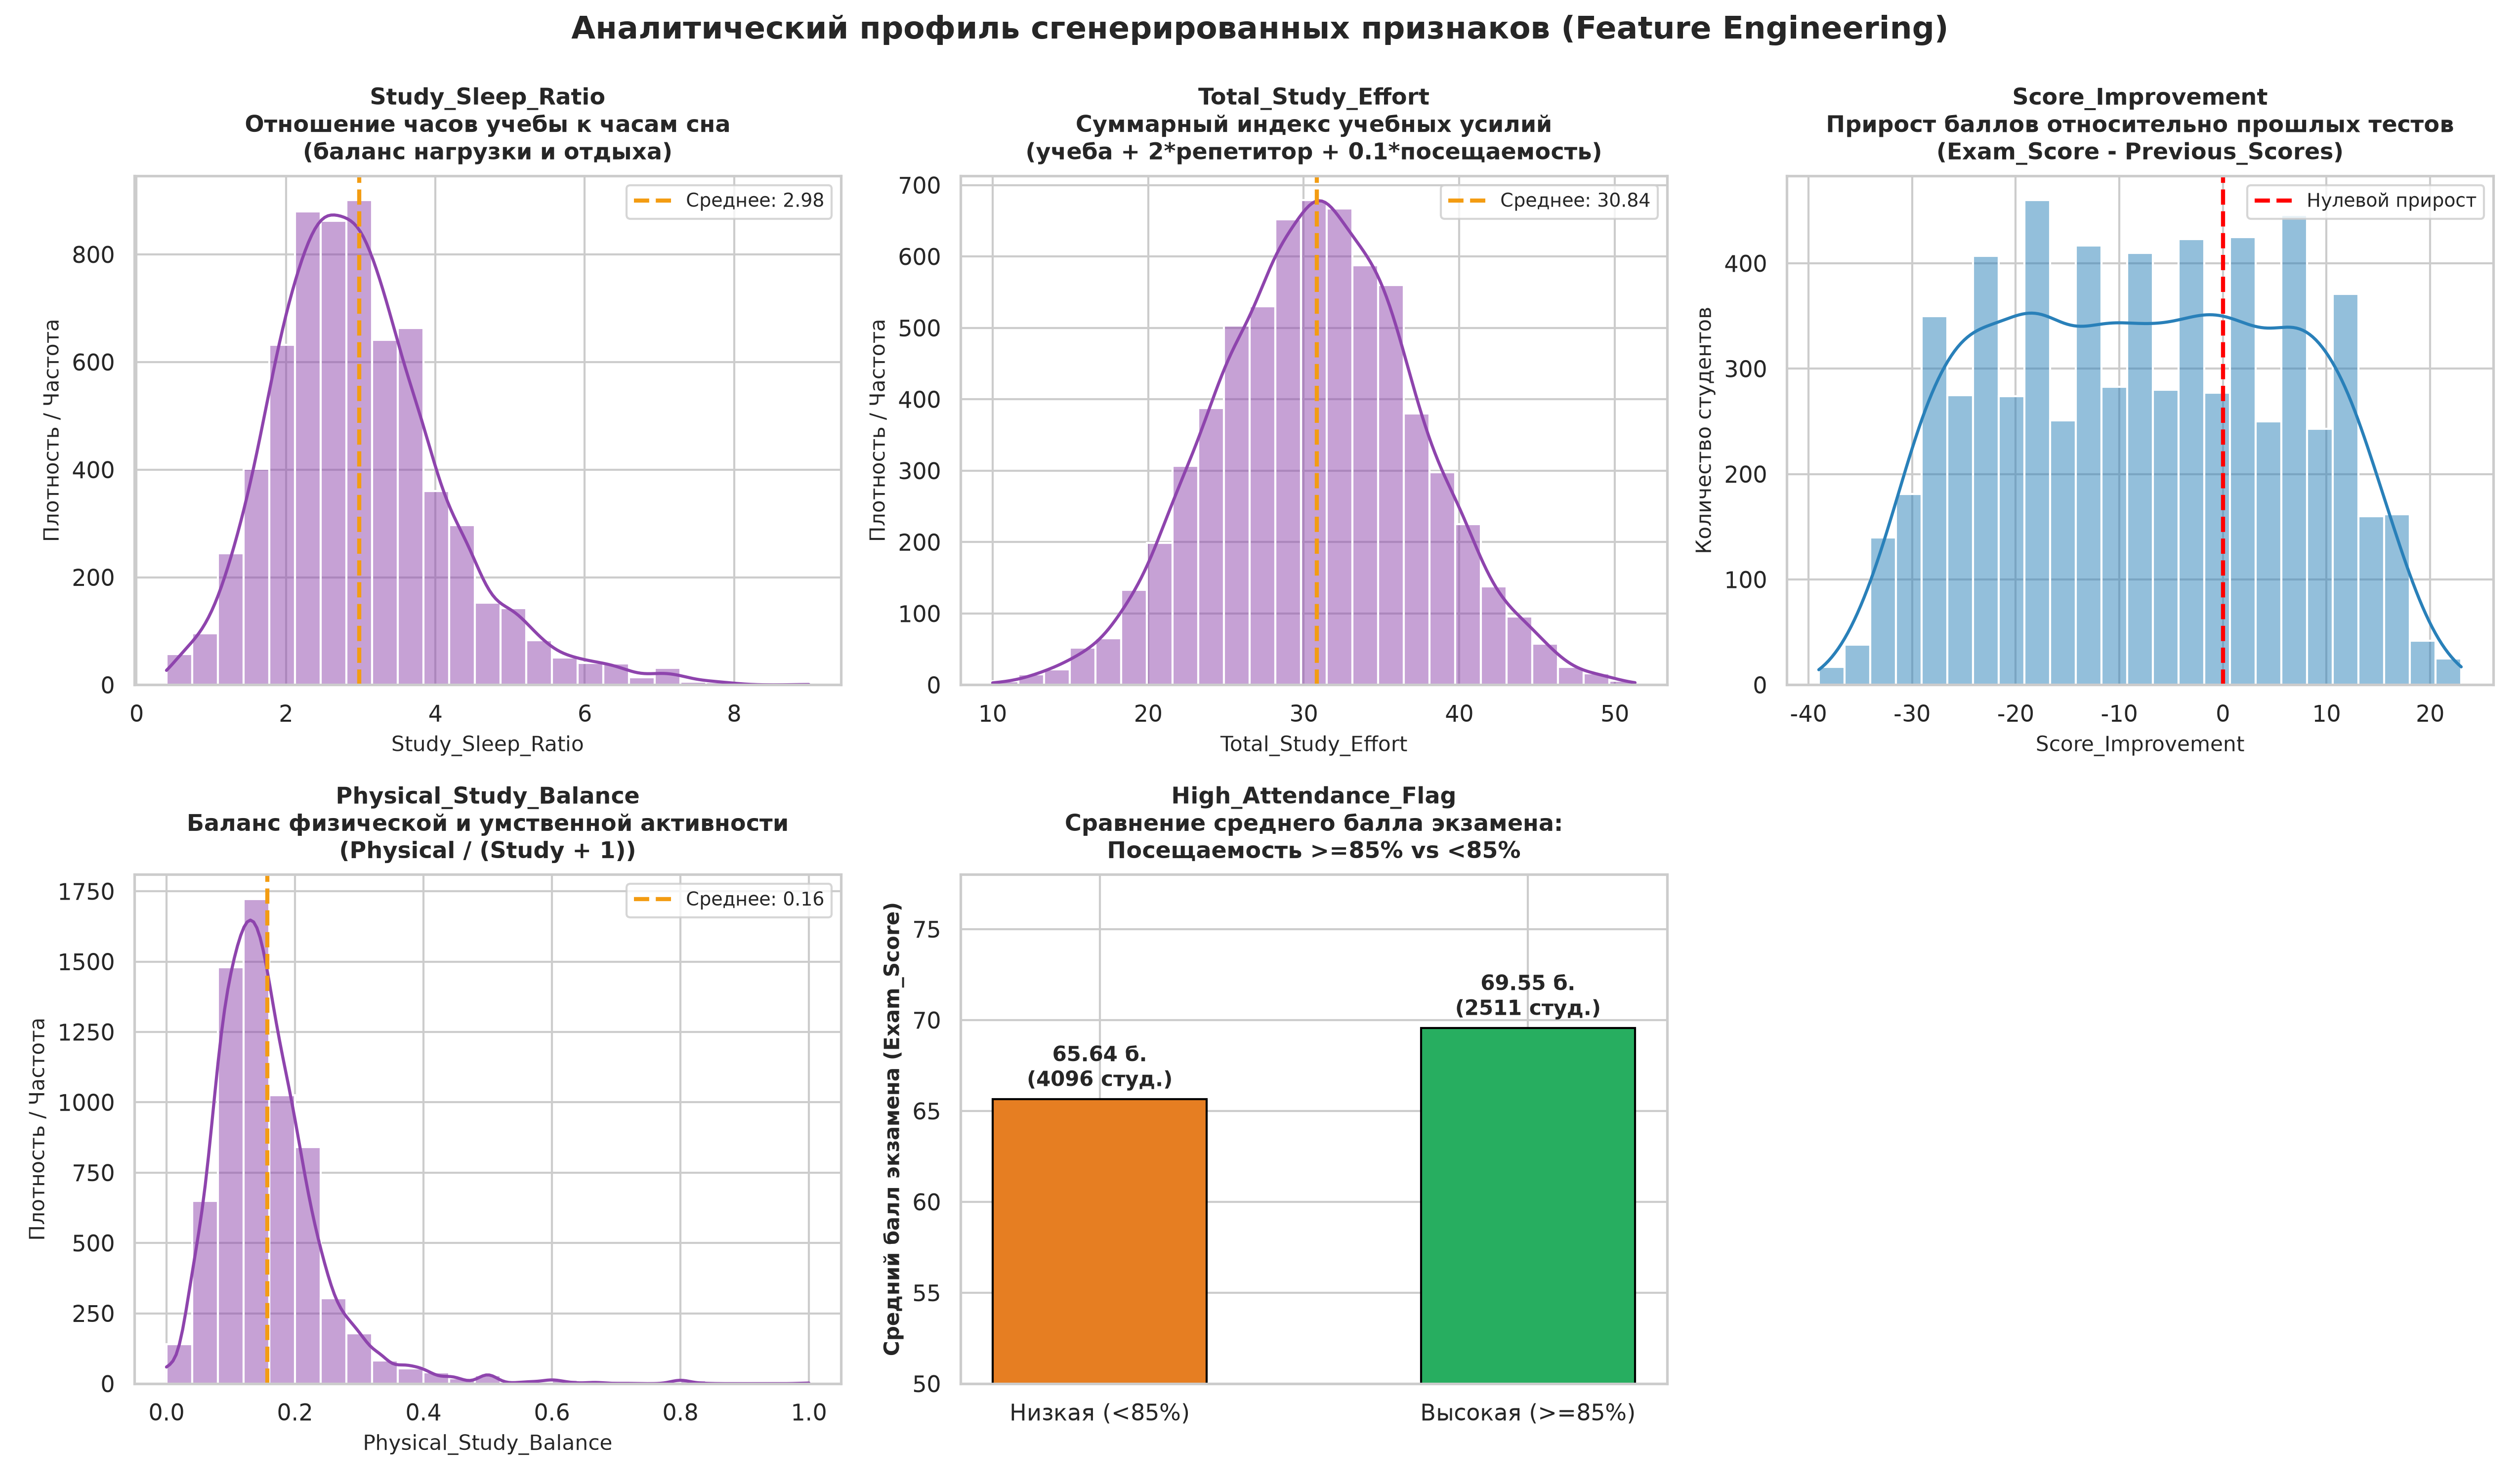
\includegraphics[width=0.92\linewidth, keepaspectratio]{images/09_feature_engineering.png}
    \caption{Аналитический профиль сгенерированных признаков (Feature Engineering)}
    \label{fig:fe}
\end{figure}

\subsection{Результаты кодирования категориальных признаков}

Выполнено преобразование всех качественных переменных:
\begin{itemize}
    \item \textbf{Бинаризация:} 5 дихотомических признаков (\texttt{Extracurricular\_Activities}, \texttt{Internet\_Access}, \texttt{Learning\_Disabilities}, \texttt{School\_Type}, \texttt{Gender}) переведены в числовые значения 0 и 1.
    \item \textbf{Порядковое кодирование (Ordinal):} 7 ранговых шкал (\texttt{Parental\_Involvement}, \texttt{Access\_to\_Resources}, \texttt{Motivation\_Level}, \texttt{Family\_Income}, \texttt{Teacher\_Quality}, \texttt{Distance\_from\_Home}, \texttt{Parental\_Education\_Level}) монотонно отображены в целочисленные ранги 0, 1, 2.
    \item \textbf{One-Hot Encoding (OHE):} номинальный признак \texttt{Peer\_Influence} преобразован в 3 бинарных столбца (\texttt{Peer\_Influence\_Negative}, \texttt{Peer\_Influence\_Neutral}, \texttt{Peer\_Influence\_Positive}).
\end{itemize}

Итоговая матрица признакового пространства расширена с 20 до \textbf{27 столбцов} при полном сохранении 6607 строк.

\subsection{Сравнительный анализ стратегий масштабирования данных}

Выполнено масштабирование 11 непрерывных признаков выборки алгоритмами \texttt{MinMaxScaler} и \texttt{StandardScaler}. В таблице~\ref{tab:scaling_stats} приведены сравнительные статистики для репрезентативных колонок.

\begin{table}[H]
    \centering
    \caption{Сравнительный анализ числовых характеристик до и после масштабирования}
    \label{tab:scaling_stats}
    \fontsize{8.5pt}{10.5pt}\selectfont
    \begin{tabularx}{\textwidth}{|>{\raggedright\arraybackslash}p{3.5cm}|>{\raggedright\arraybackslash}p{3.2cm}|c|c|c|}
        \hline
        \textbf{Признак} & \textbf{Метрика} & \textbf{Оригинал} & \textbf{MinMaxScaler} & \textbf{StandardScaler} \\
        \hline
        \texttt{Hours\_Studied} & Среднее (Mean) & 19.9718 & 0.4991 & -0.0000 \\
        & Станд. откл. (Std) & 5.9510 & 0.1860 & 1.0001 \\
        & Минимум (Min) & 4.0000 & 0.0000 & -2.6841 \\
        & Максимум (Max) & 36.0000 & 1.0000 & 2.6936 \\
        \hline
        \texttt{Attendance} & Среднее (Mean) & 79.9774 & 0.4994 & -0.0000 \\
        & Станд. откл. (Std) & 11.5475 & 0.2887 & 1.0001 \\
        & Минимум (Min) & 60.0000 & 0.0000 & -1.7302 \\
        & Максимум (Max) & 100.0000 & 1.0000 & 1.7341 \\
        \hline
        \texttt{Exam\_Score} & Среднее (Mean) & 67.1271 & 0.5079 & -0.0000 \\
        & Станд. откл. (Std) & 3.3729 & 0.2108 & 1.0001 \\
        & Минимум (Min) & 59.0000 & 0.0000 & -2.4097 \\
        & Максимум (Max) & 75.0000 & 1.0000 & 2.3343 \\
        \hline
        \texttt{Total\_Study\_Effort} & Среднее (Mean) & 30.8423 & 0.5047 & 0.0000 \\
        & Станд. откл. (Std) & 6.4088 & 0.1552 & 1.0001 \\
        & Минимум (Min) & 10.0000 & 0.0000 & -3.2524 \\
        & Максимум (Max) & 51.3000 & 1.0000 & 3.1923 \\
        \hline
    \end{tabularx}
\end{table}

На рисунке~\ref{fig:scaling} представлена сравнительная матрица $3 \times 4$ оценок ядерной плотности (KDE) для четырех признаков при трех стратегиях масштабирования.

\begin{figure}[H]
    \centering
    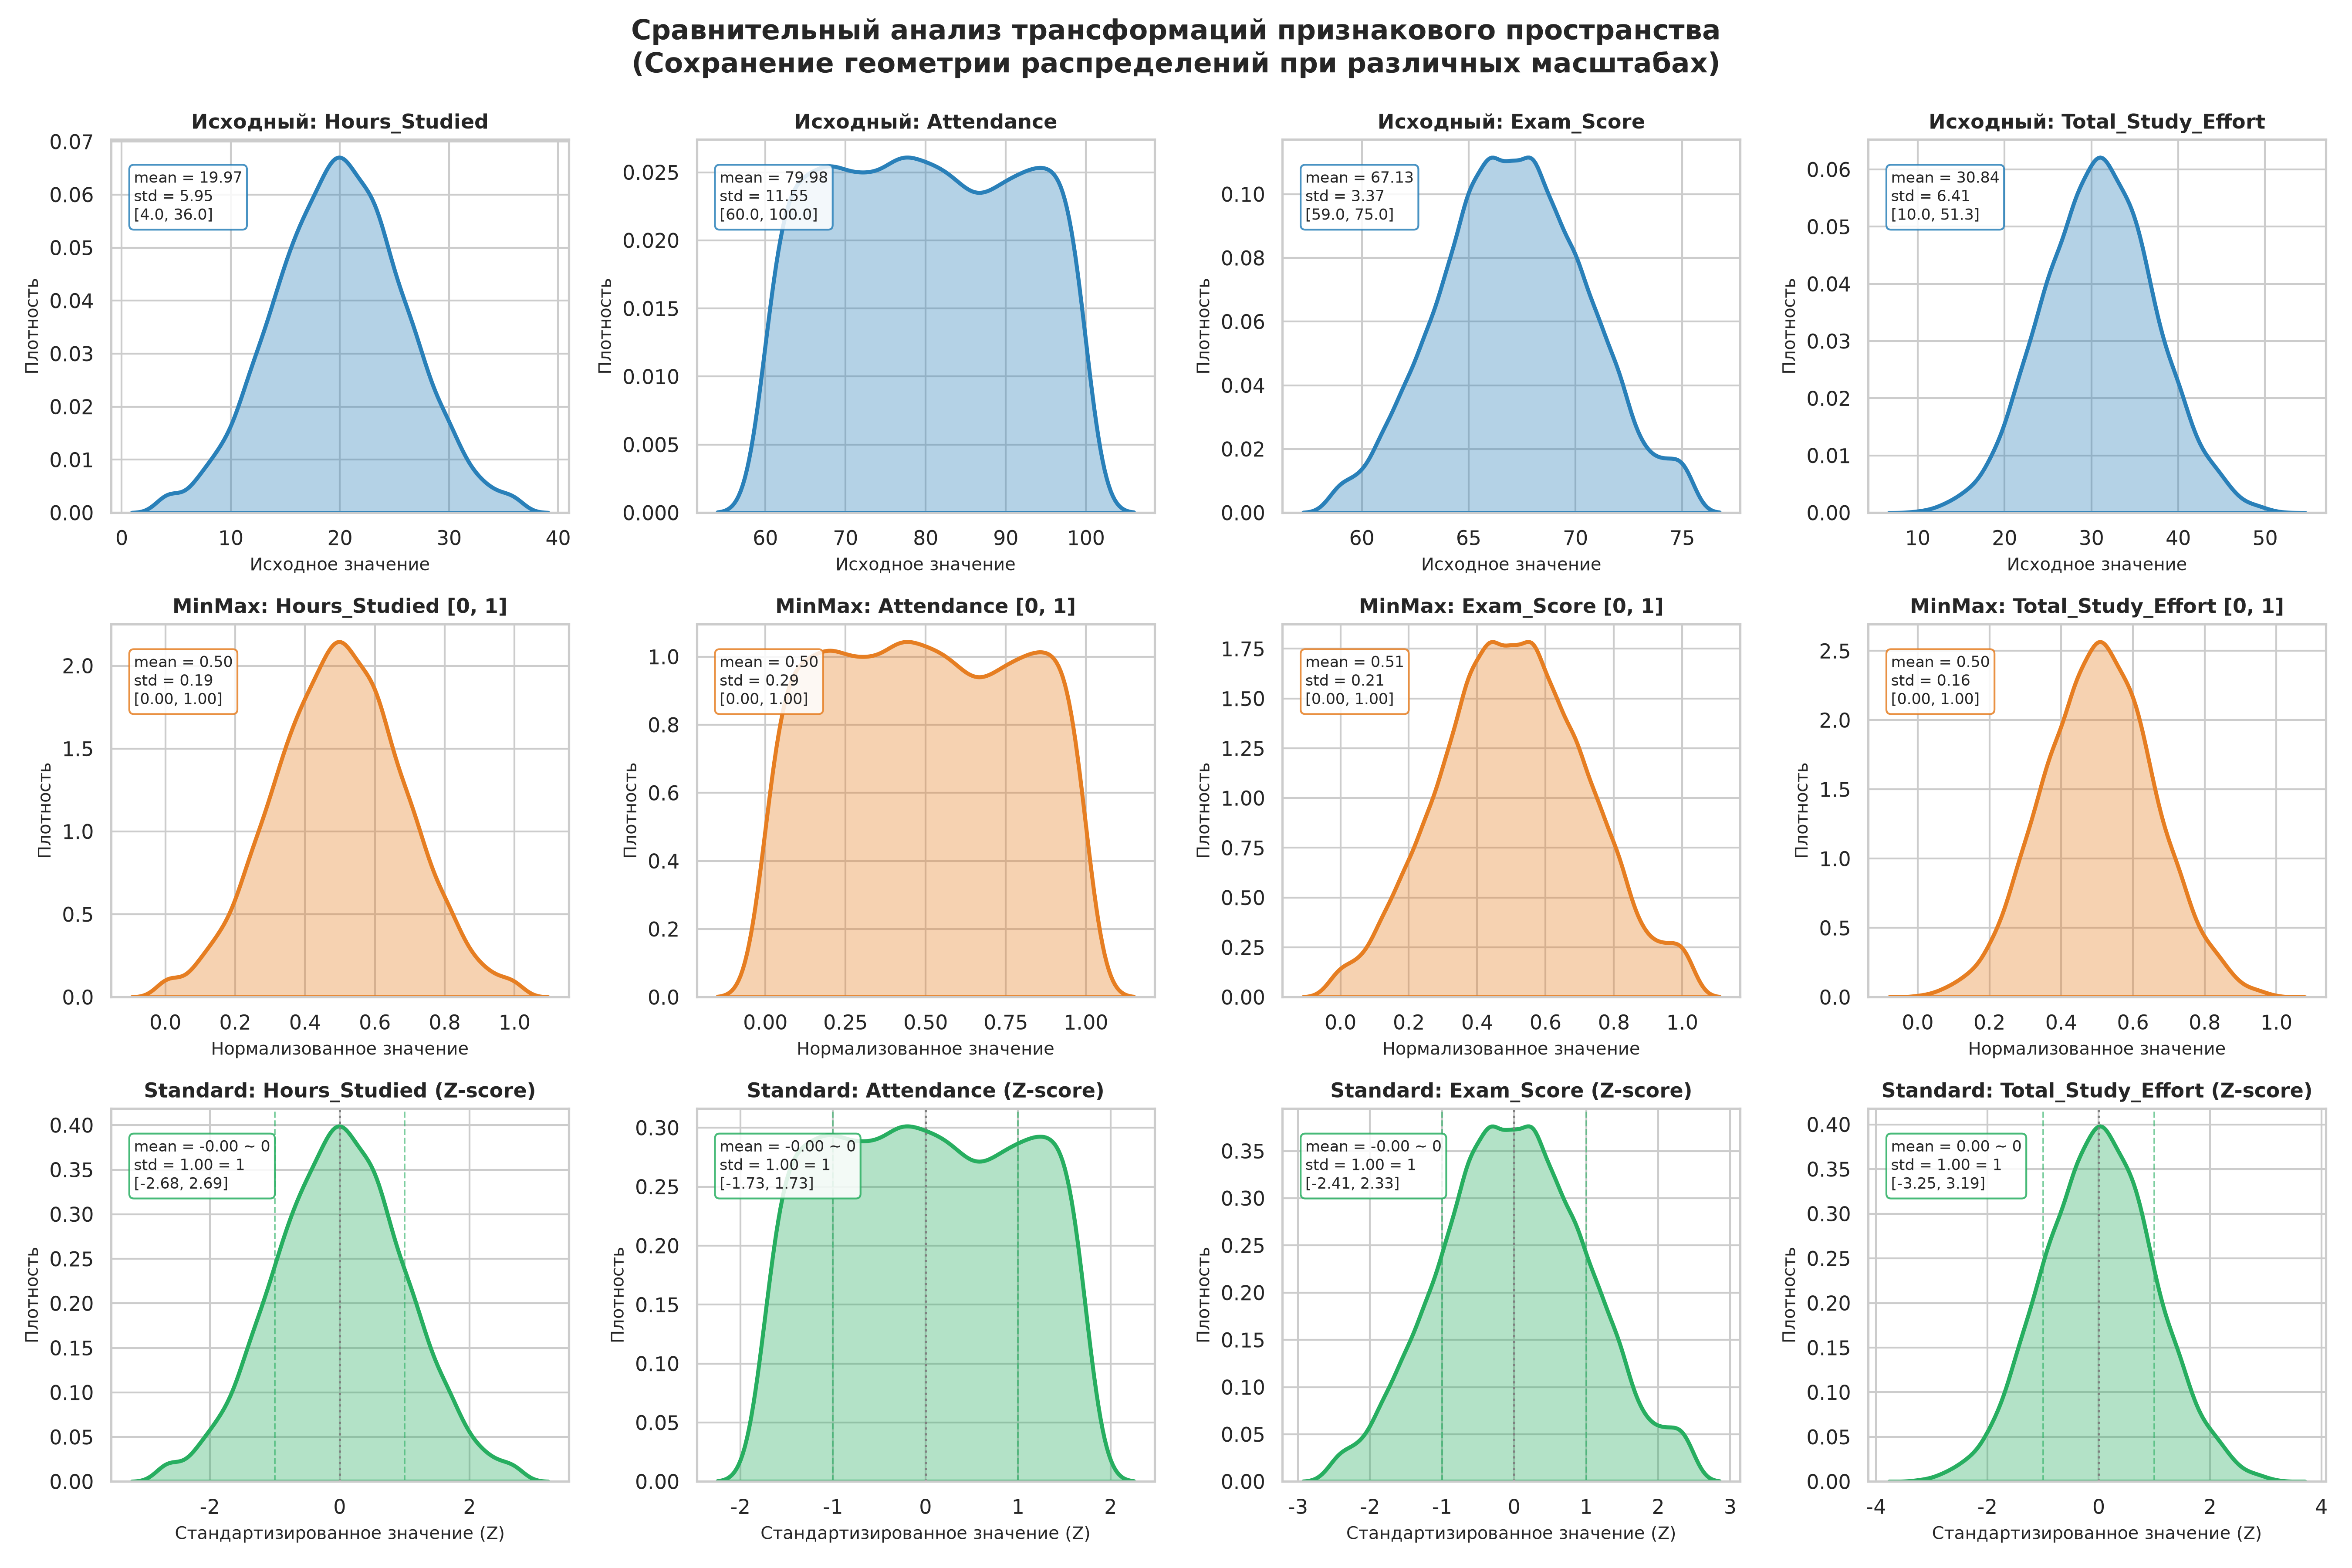
\includegraphics[width=0.95\linewidth, keepaspectratio]{images/10_scaling_comparison.png}
    \caption{Сравнительный анализ профилей плотности (KDE): Исходные vs MinMax vs Standard}
    \label{fig:scaling}
\end{figure}

\textbf{Главный вывод по масштабированию:} Проведенный анализ эмпирически подтверждает доказанную теорему: и \texttt{MinMaxScaler}, и \texttt{StandardScaler} являются строго аффинными (линейными) преобразованиями. Они приводят шкалы к нормализованным диапазонам ($[0, 1]$ и $\mu=0, \sigma=1$ соответственно), абсолютно не искажая внутреннюю топологию, асимметрию и относительное расположение квантилей исходных плотностей распределения.

% ==============================================================================
% 6 ВЫВОДЫ ПО ЛАБОРАТОРНОЙ РАБОТЕ
% ==============================================================================
\clearpage
\section{Выводы по лабораторной работе}

В ходе выполнения лабораторной работы № 2 по дисциплине «Методы машинного обучения» были достигнуты следующие академические и прикладные результаты:

\begin{enumerate}
    \item Разработан законченный модульный программный конвейер предварительной обработки структурированных данных на языке Python 3.12 с использованием современных библиотек машинного обучения (\texttt{pandas}, \texttt{numpy}, \texttt{scikit-learn}, \texttt{seaborn}, \texttt{matplotlib}).
    \item На основе статистического анализа и графической визуализации тепловыми картами выявлены скрытые пропуски в 3 категориальных атрибутах. Научно обоснована и реализована стратегия импутации модой, сохранившая 100\% объема обучающей выборки (все 6607 наблюдений) и подтвержденная контрольной тепловой картой с нулевым остаточным числом пропусков.
    \item С использованием статистического правила Тьюки ($1.5 \times IQR$) и диаграмм BoxPlot обнаружены и устранены грубая логическая аномалия в целевой переменной (\texttt{Exam\_Score} $= 101 \to 100$), а также экстремальные выбросы в переменных \texttt{Hours\_Studied}, \texttt{Exam\_Score} и \texttt{Tutoring\_Sessions}. Доказана эффективность винсоризации (\textit{clipping}), позволившей исключить тяжелые дестабилизирующие хвосты распределений без удаления наблюдений.
    \item Проведен корреляционный анализ, выявивший ведущие линейные детерминанты успеваемости студентов: посещаемость занятий ($r = 0.58$) и количество часов самостоятельной учебы ($r = 0.45$).
    \item Выполнена инженерия признаков (Feature Engineering): сконструировано 5 предметных показателей (\texttt{Study\_Sleep\_Ratio}, \texttt{Total\_Study\_Effort}, \texttt{Score\_Improvement}, \texttt{Physical\_Study\_Balance}, \texttt{High\_Attendance\_Flag}). Доказана аналитическая значимость флага дисциплины \texttt{High\_Attendance\_Flag}, показавшего разрыв в среднем балле экзамена в 5.1 единицы между группами.
    \item Реализованы корректные схемы оцифровки категориальных данных: бинаризация 5 колонок, порядковое кодирование (Ordinal Encoding) 7 колонок и One-Hot Encoding номинального признака окружения сверстников, что исключило возникновение ложного метрического порядка и расширило размерность выборки до 27 параметров.
    \item Выполнено масштабирование признакового пространства методами \texttt{MinMaxScaler} и \texttt{StandardScaler}. Теоретически и экспериментально доказана инвариантность формы ядерной оценки плотности (KDE) при линейных преобразованиях масштаба.
    \item Все требования рабочей программы лабораторной работы выполнены в полном объеме. Сформированы 4 обработанных набора данных в формате CSV и 10 графических материалов высокого разрешения (300 DPI).
\end{enumerate}

\end{document}
